%**********************************************************************************************************************************
\chapter[Sensitivity Analysis]{Sensitivity Analysis: Understanding Model Input/Output Relationship Under Uncertainty}\label{ch:gsa}
%**********************************************************************************************************************************

% Linking Paragraph
As mentioned in the introduction, describing and understanding properly the impact of model parameters variations on the model prediction are an essential part of the model development and assessment. 
This chapter presents the application of global and statistical \gls[hyper=false]{sa} to analyze the \gls[hyper=false]{feba} model in \gls[hyper=false]{trace} in order to investigate the effects of the input parameter variations.

% Focus
After first introducing in Section~\ref{sec:sa_statistical_framework} the notational convention used in the present chapter,
the proposed methodology is presented.
The methodology leverages various developments in global \gls[hyper=false]{sa} and \glsfirst[hyper=false]{fda} methods and follows three key underlying ideas.

% Overview
The first idea, presented in Section~\ref{sec:sa_time_dependent_variation}, is to reduce the dimensionality of the output space while preserving the interpretability of the results by utilizing techniques derived from \gls[hyper=false]{fda} \cite{Ramsay2005}.
Section~\ref{sec:sa_parameters_screening} introduces the second idea, which is to reduce the dimensionality of the input parameter space through screening analysis using the Morris method \cite{Morris1991,Campolongo2011}. 
The third and final idea is to investigate, quantitatively and in more detail, the effect of variation of parameters on the overall time-dependent output variation. 
This is done through variance-based SA using the Sobol’-Saltelli
method \cite{Sobol2001, Saltelli2002}, which is presented in Section~\ref{sec:sa_variance_decomposition}.

The methods are then applied to analyze the \gls[hyper=false]{feba} model in \gls[hyper=false]{trace} to understand better its inputs/outputs relationship under the assumed uncertainty on its input parameters.
The results are presented and discussed in Section~\ref{sec:sa_application_to_feba}.
Finally, Section~\ref{sec:sa_chapter_summary} closes the chapter with a summary.

%******************************************************************
\section{Statistical Framework}\label{sec:gp_statistical_framework}
%******************************************************************

Consider a general \emph{regression} problem:
\marginpar{regression problem}
Given a deterministic computer simulator (which, in essence, is a function) $f:\mathbf{x} \in \mathcal{X} \subseteq \mathbb{R}^D \mapsto \mathbb{R}$ 
evaluated at $\mathbf{DM}$, an experimental design matrix $\{\mathbf{x}_n\}_{n=1}^N$,
yielding $N$ outputs $\mathbf{y} = \{f(\mathbf{x}_n) = y_n\}_{n=1}^N$. 
the objective of regression is to compute (or \emph{predict}) the value of $f(\mathbf{x}_o)$ with $\mathbf{x}_o \notin \mathbf{DM}$.

The set $\mathcal{D} \equiv \{(\mathbf{DM}, \mathbf{y})\} = \{(\mathbf{x}_n, f(\mathbf{x}_n) = y_n)\}_{n=1}^N$ of $N$ observations is often referred to as the training data,
\marginpar{training data, training samples, and training outputs}
though the term is used interchangeably with the training outputs $\mathbf{y}$.
The experimental design matrix $\mathbf{DM}$ introduced in the previous chapter is interchangeably referred to as the training samples, inputs, or points in this chapter.
As before, the domain $\mathcal{X}$ is often rescaled such that $\mathbf{x} \in [0,1]^D$.

To evaluate $f$ at any given $\mathbf{x}_o \notin \mathbf{DM}$, the code of course can be simply run at that input.
\marginpar{emulator, surrogate model, and metamodel} 
Unfortunately, the true underlying function $f(\circ)$ that produces $y_i$ itself might be too complex and expensive to evaluate.
As such, the response surface of the function has to be reconstructed or estimated based only on small size of training data before the prediction is made.
The estimated function is chosen to be a simpler function that can be evaluated much faster (such as polynomials).
Although simpler, such an approximation should capture the most, if not all, important aspects of the inputs/outputs relationship of the true underlying function.
This simpler, approximating function is often referred to as an \emph{emulator}, \emph{surrogate model}, or \emph{metamodel}.

% Adopted framework
In this thesis, 
\marginpar{Gaussian process metamodel}
the metamodel is represented using \gls[hyper=false]{gp}, following the seminal works of Sacks et al. (\cite{Sacks1989, Sacks1989a}) and interpreted through a Bayesian perspective.
The advantages of using \gls[hyper=false]{gp} to represent an unknown function are its ability to model a complicated multi-dimensional function with limited number of parameters (\cite{Jones2009})
as well as the provision of prediction error estimate (\cite{Santner2003,Currin1991}).
Furthermore, being a statistical model based on a stochastic process, it fits the statistical calibration framework of computer model presented in the next chapter.

% Two Interpretations
The \gls[hyper=false]{gp} metamodel, like many statistical models, can be interpreted either in frequentistic sense or Bayesian sense.
\marginpar{Two interpretations}
In the frequentistic sense, the stochastic process $Y(\circ)$ is one particular realization of stochastic process (need not be Gaussian, but second-order stationary).
The prediction made at particular value of $\mathbf{x}_o$ is made based on the process as estimated according to the training data\footnote{The frequentistic case is the classical approach first developed as spatial interpolation tool in geostatistics by Krige dating back to the 1950s \cite{Krige1951} and formalized by Matheron in the 1960s \cite{Matheron1963}. In fact, Kriging model (due to Krige) is the more popular term for \gls[hyper=false]{gp} metamodel. These two terms, Kriging model and \gls[hyper=false]{gp} metamodel, will be used interchangeably in this thesis.}.
On the other hand, in the Bayesian sense, a Gaussian process is first set up as the prior for the stochastic process and the
prediction of the output at $\mathbf{x}_o$ is made based on the posterior (or conditional) process as updated by the training data.   

Both of these interpretations give an equivalent results.
The subtle difference lies in the interpretation of prediction error.
In the frequentistic case, the error is defined as the mean squared of error between the prediction made by the estimated process and (hypothetical) true process \cite{Isaaks1989};
\marginpar{prediction error}
while in the Bayesian case the error corresponds to the \emph{epistemic} uncertainty of the prediction conditional on the observed data.
That is, though the underlying computer simulation itself might be deterministic, 
the uncertainty of the prediction at $\mathbf{x}_o$ stems from the fact that the simulator was not actually run at that input and thus the output is not \emph{known}. 
The Bayesian perspective, as argued in \cite{Currin1991,Santner2003,OHagan2006}, gives more intuitive interpretation of the prediction error.
This perspective is illustrated in Fig.~\ref{fig:plot_bayesian_perspective}.
\bigtriplefigure[pos=tbhp,
								 mainlabel={fig:plot_bayesian_perspective},
			           maincaption={Gaussian process prior is equivalent to setting prior over functions. After observing data the process is updated to obtain the posterior process with a reduced uncertainties. Uncertainties are attached to each prediction made at arbitrary input outside the data (red points). Dashed lines and gray region signify the mean and $3\times \sigma$, respectively. The scales in the axes are arbitrary.},
			           mainshortcaption={Illustration of Bayesian perspective of regression and metamodeling.},%
			           leftopt={width=0.30\textwidth},
			           leftlabel={fig:plot_bayesian_perspective_1},
			           leftcaption={Prior of functions},
			           midopt={width=0.30\textwidth},
			           midlabel={fig:plot_bayesian_perspective_2},
			           midcaption={Observed data},
			           rightopt={width=0.30\textwidth},
			           rightlabel={fig:plot_bayesian_perspective_3},
			           rightcaption={Posterior function and predictions},
			           spacing={},
			           spacingtwo={}]
{../figures/chapter4/figures/plotBayesianPerspective_1}
{../figures/chapter4/figures/plotBayesianPerspective_2}
{../figures/chapter4/figures/plotBayesianPerspective_3}

\section{Describing Variation of Time-Dependent Output}\label{sec:sa_time_dependent_variation}
Illo principalmente su nos. Non message \emph{occidental} angloromanic
da. Debitas effortio simplificate sia se, auxiliar summarios da que,
se avantiate publicationes via. Pan in terra summarios, capital
interlingua se que. Al via multo esser specimen, campo responder que
da. Le usate medical addresses pro, europa origine sanctificate nos
se.
%****************************************************************
\section{Parameters Screening}\label{sec:sa_parameters_screening}
%****************************************************************

Screening methods are used to rank the importance of the model parameters using a relatively small number of model evaluations \cite{Saltelli2004}.
However, they tend to simply give qualitative measures.
That is, meaningful information resides in the rank itself but not in the exact importance of the parameters with respect to the output. 
Screening is particularly valuable in the early phase of a SA to identify the noninfluential parameters of a model,
which then could be safely excluded from further detailed analysis. 
This step is important to reduce the size of the problem especially if more expensive methods are to be applied at the subsequent steps. 
In this work, attention was paid to a particular screening method proposed by Morris \cite{Morris1991} with an extension proposed by Campolongo et al. \cite{Campolongo2011}.

%----------------------------------------------------------------------------
\subsection{Elementary Effects and One-at-a-Time Design}\label{sub:sa_ee_oat}
%----------------------------------------------------------------------------

% Elementary effect definition
Consider a mathematical model $f: \bm{x} \in [0,1]^D \mapsto y = f(\bm{x}) \in \mathbb{R}$, 
where $\bm{x} = (x_1, x_2, \dots,x_D)$ is a vector of input parameters.
The elementary effect of the $d$-th parameter on $f$ is defined as
\marginpar{elementary effect}
\begin{equation}
  EE_d = \frac{f(x_1, \dots, x_d+\Delta,\dots,x_D) - f(x_1, \dots, x_d,\dots,x_D)}{\Delta}
\label{eq:elementary_effect}
\end{equation}
or more concisely,
\begin{equation}
  EE_d = \frac{f(\bm{x} + \Delta \cdot \bm{e}_d) - f(\bm{x})}{\Delta}
\label{eq:elementary_effect_concise}
\end{equation}
where $\bm{e}_d$ is the $d$-th basis vector of the input parameter space;
and $\Delta$, the grid jump, is chosen such that $\mathbf{x} + \Delta \cdot \bm{e}_d$ is still in the specified domain of the parameter space, i.e., $[0,1]^D$; 
$\Delta$ is a value in $\{\frac{1}{p-1}, \dots, 1 - \frac{1}{p-1}\}$, 
where $p$ is the number of (discretization) levels that partition the model parameter space into a uniform grid of points where the model can be evaluated. 
For a given $p$, the grid constructs a finite distribution of $p^{D-1}[p - \Delta(p-1)]$ elementary effects for each input parameter.

% OAT Experimental Design
The elementary effect distributions for each of the input parameters,
evaluated across discretized input parameter space, 
\marginpar{\gls[hyper=false]{oat} experimental design}
provide useful information on the importance of a parameter on the output.
Unfortunately, an exhaustive evaluation of all elementary effects for a given discretization levels suffers from a curse of dimensionality especially for numerous parameters and/or for reasonably fine discretization level\footnote{for $p = 8$ and $D = 20$ the total number of evaluations for exhaustive computation of all $EE$s is $\approx 6 \times 10^{17}$ for each parameter}.
Consequently, a class of design of experiment that only change one parameter at a time (\gls[hyper=false]{oat}) are devised to estimate the statistics of the distributions.
  
% Trajectory OAT Design
The key idea behind the original Morris method is in initiating the model evaluations from various \textit{nominal} points, $\bm{x}$,
\marginpar{trajectory OAT design}
randomly selected over the grid and then gradually advancing one grid jump, perturbing one parameter at a time,
making a perturbed point as the base point for the next perturbation.
The order of perturbation (i.e., which dimension to perturb first) and the direction of the perturbation (i.e., whether it is added or subtracted) are also randomized between replications.
As such, different replication generates different starting nominal point as well as different order and sign (but with the same size) of perturbation.
The \gls[hyper=false]{oat} experimental design complemented with this requirement is known as the trajectory design \cite{Ruano2012}.
Fig.~\ref{fig:ch3_plot_oat_illustration_1} illustrates a trajectory design with $4$ replications in a two-dimensional input parameter space discretized in $6$ levels .
\normdoublefigure[pos=tbhp,
                  mainlabel={fig:ch3_plot_oat_illustration},
                  maincaption={Illustration of One-at-a-Time (OAT) design constructed using trajectory scheme (left) and radial scheme (right) each with 4 replications. The trajectory design is discretized in 6 levels, while the number of levels is irrelevant for radial design. Filled circles are the nominal or the starting point (for the trajectory) or the base (for the radial) points and crosses are the perturbed levels.},%
									mainshortcaption={Illustration of One-at-a-Time (OAT) design using trajectory and radial schemes.},
                  leftopt={width=0.45\textwidth},
                  leftlabel={fig:ch3_plot_oat_illustration_1},
                  leftcaption={Trajectory scheme},
                  %leftshortcaption={},%
                  rightopt={width=0.45\textwidth},
                  rightlabel={fig:ch3_plot_oat_illustration_2},
                  rightcaption={Radial scheme},
                  %rightshortcaption={},
                  %spacing={\hfill}
                 ]
{../figures/chapter3/figures/plotOATIllustration_1}
{../figures/chapter3/figures/plotOATIllustration_2}

To remove the requirement to specify a method-specific parameter $p$ (the number of levels),
\marginpar{radial OAT design}
Campolongo et al.\cite{Campolongo2011} proposed to use a radial scheme coupled with Sobol' quasirandom sequence.
In a single replication of this particular OAT design, 
each parameter is perturbed relative to a \textit{base/nominal} point 
which is not required to be located on a predetermined grid.
The size and sign of the perturbation is also allowed to vary from parameter to parameter in different replication.
As such, radial design implicitly incorporates several additional possible sources of variation in the method 
that can potentially bias the estimation of elementary effects.
Because the size of parameter perturbations varies, the definition of the elementary effects is slightly changed to,
\marginpar{elementary effect for radial design}
\begin{equation}
EE_d = \frac{f(\bm{x} + \Delta x_d \cdot \bm{e}_d) - f(\bm{x})}{\Delta x_d}
\end{equation}
where now each parameter at each design replication has its corresponding perturbation size $\Delta x_d \in [-1,1]$ such that $x_d + \Delta x_d \in [0,1]$.

An illustration of a radial design in a two-dimensional input parameter space with $4$ nominal/base points is shown in Fig.~\ref{fig:ch3_plot_oat_illustration_2}.
 
%-------------------------------------------------------------------------------------------------
\subsection{Statistics of Elementary Effects and Sensitivity Measures}\label{sub:sa_ee_statistics}
%-------------------------------------------------------------------------------------------------

% Mean of the elementary effects
Consider now that an $N_R$ number of elementary effects associated with the $d$-th parameter have been sampled from the finite distribution of $EE_d$,
using a \gls[hyper=false]{oat} design with $N_R$ replications.
The statistical summary of sampled $EE_d$ based on a given number of OAT design replications generated using either the trajectory or the radial design can be calculated.
The first is the arithmetic mean defined as,
\marginpar{the mean of the (sampled) elementary effects}
\begin{equation}
	\mu_d = \frac{1}{N_R} \sum_{r = 1}^{N_R} EE^r_d
	\label{eq:sa_morris_mu}
\end{equation} 
where $EE^r_d$ is the elementary effect of the $d$-th parameter of the $r$-th replication.
The mean gives the global influence of the $d$-th parameter on the chosen output $f$.

% Standard deviation of the elementary effects
The second statistical summary of interest is the standard deviation of the (sampled) elementary effects for input parameter $x_d$,
\marginpar{the standard deviation of the (sampled) elementary effects}
\begin{equation}
	\sigma_d = \sqrt{\frac{1}{N_R} \sum_{r = 1}^{N_R} (EE^r_d - \mu_d)^2}
	\label{eq:sa_morris_sd}
\end{equation} 
The standard deviation gives an indication of the presence of nonlinearity and/or interactions between the $d$-th input parameter and the others.

% Mean of absolute values of the elementary effects
In cases where $f$ is a non-monotonic function,
the sign of $EE_d$ may change according to the change of the output,
and cancellation effects on the estimation of $\mu_d$ might occur .
To circumvent this issue,
Campolongo et al.~\cite{Campolongo2011} proposed to take the absolute values of the sampled elementary effects.
It is defined as,
\marginpar{the mean of the (sampled) absolute elementary effects}
\begin{equation}
	\mu^*_d = \frac{1}{N_R} \sum_{r = 1}^{N_R} |EE^r_d|
	\label{eq:sa_morris_mustar}
\end{equation}
Note that although the overall sign of the output perturbation is lost by using this measure,
its use is justified if the input parameters are to be ranked based on a single importance measure.

% Interpretation and importance classification
The aforementioned statistical summaries, when evaluated over a large number of replications $N_R$,
can provide global sensitivity measures of the importance of each input parameter.
\marginpar{input parameter importance classification}
As indicated by Morris \cite{Morris1991}, there are three possible categories of parameter importance based on those statistics:
\begin{enumerate}
	\item Parameters with noninfluential effects, i.e., the parameters that have relatively small values of both $\mu_d$ (or $\mu^*_d$) and $\sigma_d$;
	The parameter has a negligible overall effect on the model output.
	\item Parameters with linear and/or additive effects, i.e., the parameters that have relatively large value of $\mu_d$ (or $\mu^*_d$) and relatively small value of $\sigma_d$.
	The small value of $\sigma_d$ and the large value of $\mu_d$ (or $\mu^*_d$) indicate that the variation of elementary effects across replications is small while the magnitude of the effect itself is consistently large for the perturbations in the parameter space.
	\item Parameters with nonlinear and/or interaction effects, i.e., the parameters that have a relatively small value of $\mu_d$ (or $\mu^*_d$) and a relatively large value of $\sigma_d$.
	Opposite to the previous case, a small value of $\mu_d$ (or $\mu^*_d$) indicates that the aggregate effect of perturbation is relatively small (or in the case of $\mu_d$, can be close to zero) while a large value of $\sigma_d$ indicates that the variation of the effect is large; the effect can be large or negligibly small depending on the values of the other parameters at which the model is evaluated.
	Such large variation is a symptom of nonlinear effects and/or parameter interaction.
\end{enumerate}

% Classification and qualitative measure
Such classification makes parameter importance ranking and, in turn, screening of noninfluential parameters possible.
However, the procedure is done rather qualitatively, and this is illustrated in Fig.~\ref{fig:ch3_importance_classification}, 
which depicts a typical parameter classification derived from visual inspection of the elementary effects statistics on the $\sigma$ vs. $\mu^*$ plane.
The notions of influential and noninfluential parameters are based on the relative locations of those statistics in the plane.
Typically, the noninfluential ones are clustered closer to the origin (relative to the more influential ones) with a pronounced boundary such as the one depicted in Fig.~\ref{fig:ch3_importance_classification}. 
Admittedly, if these statistics are spread somewhat uniformly across the plane, 
the distinction would be more ambiguous and problematic\footnote{In such a case, a more advanced classification such as the ones based on clustering techniques might be helpful to identify a finer structure of the parameters importance.}.
Furthermore, for a parameter with a large value of both $\mu^*$ and $\sigma$,
the method cannot distinguish between nonlinearity effect from parameter interaction effect on the output.

\begin{figure}[bth]
	\centering
	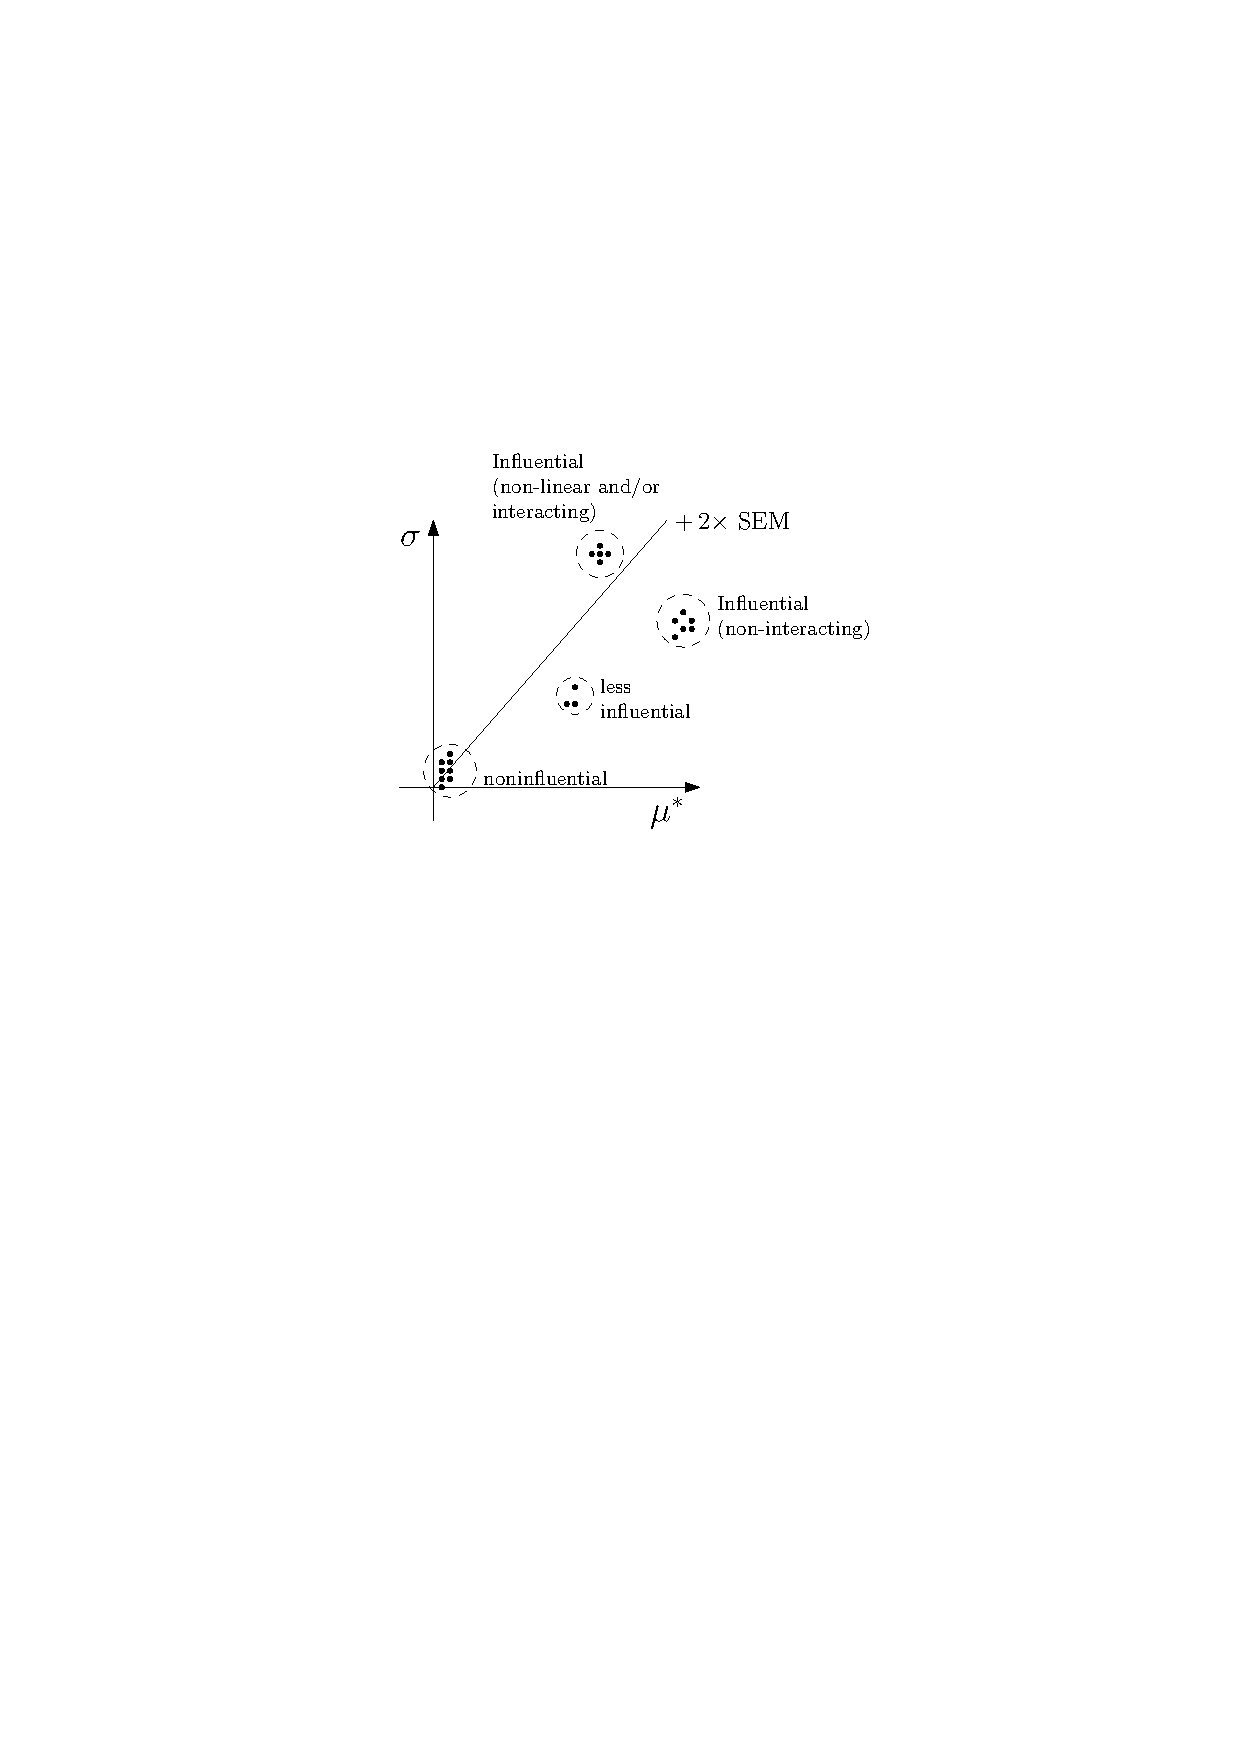
\includegraphics[scale=0.80]{../figures/chapter3/ipe/importance_classification}
	\caption[Illustration of a typical parameter importance classification based on Morris screening method]{Illustration of a typical parameter importance classification obtained from the Morris screening method. The importance of each parameter relative to the other ones is defined with respect to its location on the $\sigma - \mu^*$ plane. Each dot represents a parameter, and the line corresponds to twice the standard error of the mean (SEM) indicating the relative magnitude of the standard deviation to the mean.}\label{fig:ch3_importance_classification}
\end{figure}

\section{Variance Decomposition}\label{sec:variance_decomposition}
Illo principalmente su nos. Non message \emph{occidental} angloromanic
da. Debitas effortio simplificate sia se, auxiliar summarios da que,
se avantiate publicationes via. Pan in terra summarios, capital
interlingua se que. Al via multo esser specimen, campo responder que
da. Le usate medical addresses pro, europa origine sanctificate nos
se.
\section{Implementation}\label{sec:sa_implementation}

An implementation of the Morris method and a Monte Carlo method to estimate the main- and total-effect sensitivity indices has been developed using the Python \cite{PCT2017} programming language 
for the purpose of this work, to allow for well-controlled parametric and convergence studies.
The implementation follows a black box approach of sensitivity analysis. 
It deals with the generation of design of experiment (which is used to evaluate the model or code) and the post-processing of output to obtain the select measures of sensitivity.
In the following, the basic procedures that underlie the implementation of both methods are laid out.
More details on the programming aspects of the implementation (the so-called \texttt{gsa-module}) can be found in Appendix~\ref{app:gsa_module}.

\subsection{The Morris Method}\label{sub:sa_morris}

The implementation of the Morris method (see Section~\ref{sub:sa_ee_oat}) follows four sequential steps. 
\textsc{First}, an OAT design matrix consisting of $N_R$ replications is created by randomly sampling the nominal (base) points as well as the perturbed points for each parameter.
A replication in an OAT design consists of $1$ nominal point with $D$ (number of dimen~sions/parameters) additional perturbed points.
In each of the perturbed points, only one parameter change its value relative to the base.
Different replication yields different nominal point and the associated perturbed points.

\textsc{Second}, each point in the design matrix is scaled to the corresponding point in the $D$-dimensional parameter space of the model parameters.

\textsc{Third}, the model is evaluated for each (rescaled) point in the design matrix. The total number of model evaluations for a given design matrix of size $N_R$ is $N_R \times (D + 1)$.

\textsc{Fourth} and finally, the $N_R$ elementary effects $EE_d$ for each parameter and each trajectory are computed for a selected \gls{qoi}.
Their statistical summaries ($\mu_d$, $\mu_d^*$, $\sigma_d$) are then computed, 
and the ranking of the parameters can be constructed based on $\mu_d^*$ for a selected \gls{qoi}.
The $\mu_d^*$ can be directly used to rank the parameters to systematically identify 
and screen out noninfluential parameters (low $\mu_d^*$) from the relatively influential ones (high $\mu_d^*$)~\cite{Campolongo2007}.

\subsection{The Sobol'-Saltelli Method}\label{sub:sa_sobol_saltelli}

In principle, the estimation of the Sobol' indices defined by Eqs.~(\ref{eq:sa_main_effect_index}) and (\ref{eq:sa_total_effect_index}) can be directly carried out using \gls{mc} simulation.
\marginpar{brute force \\ Monte Carlo}
The most straightforward, though rather naive, 
implementation of \gls{mc} simulation to conduct the estimation is using two nested loops for the computation of the conditional variances and expectations appearing in both equations.

In the estimation of the main-effect index of parameter $x_d$, for instance, 
the outer loop samples values of $X_d$ while the inner loop samples values of $\mathbf{X}_{\sim d}$ (anything else other than $x_d$).
These samples, in turn, are used to evaluate the model output.
In the inner loop, the mean of the model output (for a given value of $X_d$ but over many values of $\mathbf{X}_{\sim d}$) is taken. 
Afterward, in the outer loop, the variance of the model output (over many values of $X_d$) is taken.
This approach can easily become prohibitively expensive as the nested structure requires $N^2$ model evaluations \emph{per input dimension} for either the main-effect and total-effect indices, 
while $N$ (the size of \gls{mc} samples) are typically in the range of $10^2 - 10^4$ for a reliable estimate. 

Sobol' \cite{Sobol2001} and Saltelli \cite{Saltelli2002} proposed an alternative approach that circumvent the nested structure of \gls{mc} simulation to estimate the indices.
The formulation starts by expressing the the expectation and variance operators in their integral form 
and ends with different possible \gls{mc} estimators for both sensitivity indices.
A detailed derivation of the integral form and the origin of the estimator can be found in Appendix~\ref{app:sobol_saltelli}. 

The computational cost associated with the estimation of all the main-effect and total-effect indices using the Sobol'-Saltelli method is $N \times (D + 2)$ code runs,
\marginpar{computational cost: \\ brute force Monte Carlo vs. Sobol'-Saltelli}
where $N$ is the number of \gls{mc} samples and $D$ is the number of parameters.
Compare this to the cost of brute force Monte Carlo of $2 \times D \times N^2$ code runs to estimate all the main-effect and total-effect sensitivity indices. 

As an additional comparison, the cost for Morris method to compute the statistics of elementary effect is $N_R \times (D + 1)$ code runs,
\marginpar{computational cost: \\ Morris vs. Sobol'-Saltelli}
where $N_R$ is the number of OAT design replications.
In either methods, the number of samples $N$ (in the case of the Sobol'-Saltelli method) and replications $N_R$ (in the case of the Morris method)
determines the precision of the estimates.
A larger number of samples (and replications) increases the precision.
Note, however, that in practice the typical number of Morris replications is between $10^1 - 10^2$~\cite{Saltelli2010}, 
while the number of \gls{mc} samples for the Sobol' indices estimation amounts to $10^2 - 10^4$~\cite{Sobol2001}.

As it was the case for the Morris method, an implementation of the Sobol'-Saltelli method is also part of \texttt{gsa-module} python3 package (see Appendix~\ref{app:gsa_module} for detail). 
For $N$ number of \gls{mc} samples and $D$ number of model parameters, the \gls{mc} simulation procedure to estimate the sensitivity indices follows the sampling and resampling approach adopted in~\cite{Sobol2001,Saltelli2002,Homma1996} described in the following.

\textsc{First}, generate two $N \times D$ independent random samples from a uniform independent distribution in $D$-dimension, $[0,1]^D$:
\begin{equation}
A = 
\begin{pmatrix}
a_{11}  & \cdots  & a_{1D}\\
\vdots	& \ddots & \vdots\\
a_{N1}  & \cdots  & a_{ND}\\
\end{pmatrix}
;\quad B = 
\begin{pmatrix}
b_{11}  & \cdots  & b_{1D}\\
\vdots	& \ddots & \vdots\\
b_{N1}  & \cdots  & b_{ND}\\
\end{pmatrix}
\label{eq:ss_two_samples}
\end{equation}

\textsc{Second}, construct $D$ additional design of experiment matrices where each matrix is matrix $A$ with the $d$-th column substituted by the $d$-th column of matrix $B$:\begin{equation}
  \begin{split}
  & A_{B}^1 = 
  \begin{pmatrix}
    b_{11}  & \cdots  & a_{1D}\\
    \vdots	& \ddots & \vdots\\
    b_{N1}  & \cdots  & a_{ND}\\
  \end{pmatrix} \\
  & A_{B}^{d} = 
  \begin{pmatrix}
    a_{11}  & \cdots & b_{1d} & \cdots & a_{1D}\\
    \vdots	& \cdots & \vdots & \cdots & \vdots\\
    a_{N1}  & \cdots & b_{Nd} & \cdots & a_{ND}\\
  \end{pmatrix} \\
  & A_{B}^{D} = 
  \begin{pmatrix}
    a_{11}  & \cdots  & b_{1D}\\
    \vdots	& \ddots & \vdots\\
    a_{N1}  & \cdots  & b_{ND}\\
  \end{pmatrix}
  \end{split}
\label{eq:ss_sampling_resampling}
\end{equation}

\textsc{Third}, rescale each element in the matrices of samples to the actual values of model parameters according to their actual range of variation through iso-probabilistic transformation.

\textsc{Fourth}, evaluate the model multiple times using input vectors that correspond to each row of $A$, $B$, and all the $A_B^d$.

\textsc{Fifth} and finally, extract the \gls{qoi}s from all the outputs and recast them as vectors.
The main-effect and total-effect indices are then estimated using the estimators described below.

For the main-effect sensitivity index, two estimators are considered.
One is proposed by Saltelli~\cite{Saltelli2002}, and the other, as an alternative, is proposed by Janon et al~\cite{Janon2014}.
The latter proved to be more efficient, especially for a large variation around a parameter estimate~\cite{Iooss2015,Janon2014}.

The general form of main-effect sensitivity index estimator is
\marginpar{Main-effect sensitivity index estimators}
\begin{equation}
  \widehat{S}_d = \frac{\frac{1}{N}\sum_{n=1}^N f(B)_n \cdot f(A_B^d)_n - \mathbb{E}^2[Y]}{\mathbb{V}[Y]}
\label{eq:ss_main_effect_estimator}
\end{equation}
where and $\mathbb{E}^2[Y]$ and $\mathbb{V}[Y]$ are as prescribed in Table~\ref{tab:ss_main_effect_estimator}.
where the subscript $n$ corresponds to the row of the sampled model parameters 
such that $f(B)_n$ is the model output evaluated using inputs taken from the $n$-th row of matrix $B$ 
and $f(A_B^d)_n$ is the model output evaluated using inputs taken from the $n$-th row of matrix $A_B^D$.
The \gls{mc} estimator for the second term in the numerator and for the denominator differ for the two considered estimators given in Table~\ref{tab:ss_main_effect_estimator}.
%The first term in the numerator of Eq.~(\ref{eq:ss_main_effect_estimator}) is the same for both Saltelli and Janon et al. estimators and is given by
%\begin{equation}
%  \int \int f(\mathbf{x}^{\prime}_{\sim d}, x_d) f(\mathbf{x}_{\sim d}, x_d) d\mathbf{x}^{\prime}_{\sim d} d\mathbf{x}_{\sim d} \approx \frac{1}{N}\sum_{n=1}^N f(B)_n \cdot f(A_B^d)_n
%\label{eq:ss_first_term}
%\end{equation}

\begin{table}[h]
	\myfloatalign
	\caption[Monte Carlo estimators to estimate the main-effect indices]{Two \gls{mc} estimators for the terms in Eq.~(\ref{eq:ss_main_effect_integral}) to estimate the main-effect indices (the sum is taken implicitly over all samples $N$)}
	\label{tab:ss_main_effect_estimator}
	\begin{tabularx}{\textwidth}{Xll} \toprule
		\tableheadline{Estimator}         & $\mathbb{E}^2[Y] = \left( \int f d\mathbf{x}\right)^2$          & $\mathbb{V}[Y] = \int f^2 d\mathbf{x} - \left( \int f d\mathbf{x}\right)^2$ \\ \midrule 
		Saltelli \cite{Saltelli2002}      & $\frac{1}{N} \sum f(A)_n \cdot f(B)_n$                          & $\frac{1}{N}\sum f(A)_n^2-\left(\frac{1}{N}\sum f(A)_n\right)^2$  \\[0.75cm]
		Janon et~al.~\cite{Janon2014}     & $\left(\frac{1}{2N} \sum f(B)_n + f(A_B^d)_n\right)^2$          & $\frac{1}{2N} \sum f(B)_n^2 + f(A_B^d)_n^2$ \\
                                      &                                                                 & $\quad -\left(\frac{1}{2N} \sum f(B)_n^2 + f(A_B^d)_n^2\right)^2$ \\
		\bottomrule
	\end{tabularx}
\end{table}

To estimate the total-effect sensitivity indices, the Jansen estimator~\cite{Jansen1999} is recommended in~\cite{Saltelli2010a}.
\marginpar{Total-effect sensitivity index estimators}
The estimator reads
\begin{equation}
  \widehat{ST}_d = \frac{\frac{1}{2N}\sum_{n=1}^{N}\left(f(A)_n - f(A_B^d)_n\right)^2}{\mathbb{V}[Y]}
\label{eq:ss_jansen_estimator}
\end{equation}
where $\mathbb{V}[Y]$ is estimated by the Saltelli et al. estimator as prescribed in Table~\ref{tab:ss_main_effect_estimator}.

%*************************************************************************************************************************************************
\chapter[Bayesian Calibration]{Bayesian Calibration of Computer Model: Bridging Model \& Data under Uncertainty}\label{ch:bayesian_calibration}
%*************************************************************************************************************************************************

% Link paragraph
In Chapter~\ref{ch:gsa}, a sensitivity analysis method was employed to better understand the inputs/outputs relationship in a computer simulation model with uncertain inputs.
The method was also able to reduce the size of the problem by screening out non-influential inputs.
Chapter~\ref{ch:gp_metamodel} then developed a fast approximation to evaluate the output at any given input point, in anticipation of the high cost of the calibration approach presented in this chapter.
The respective methods were exemplified by their application to a \gls[hyper=false]{trace} reflood simulation model whose inputs were uncertain, as assumed in Chapter~\ref{ch:trace_reflood}.

% Focus paragraph
This chapter deals with a statistical framework for calibrating the inputs of a simulation model.
The framework casts the calibration problem as a statistical inverse problem where the initial (prior) uncertainties of the inputs are updated based on available observed data.
It considers the a priori uncertainties in the inputs and in the experimental data, as well as the possible bias of the model.
The inputs uncertainties are then coherently updated via the Bayes' theorem resulting in an updated (posterior) probability density.
The updated uncertainty of the inputs can then be propagated through the simulation model to quantify the prediction uncertainty.

% Overview paragraphs
Section~\ref{sec:bc_statistical_framework} first presents the statistical framework for the problem of computer model calibration, 
while Section~\ref{sec:bc_modular} elaborates further the formulation of the calibration problem through probabilistic modeling of the data-generating process.
This results in the formulation of the posterior probability density.
The posterior density is often a complex highly multi-dimensional function, which makes it difficult to work with.
Section~\ref{sec:bc_mcmc} presents a simulation method (i.e., \glsfirst[hyper=false]{mcmc} simulation) to directly generates representative samples from the posterior density.
These samples can be used to approximate the posterior density or for uncertainty propagation.
Important aspects of analyzing samples of a Markov chain are presented in Section~\ref{sec:bc_mcmc_diagnostic}.
Section~\ref{sec:bc_application_to_feba} then discusses the application of the approach to the \gls[hyper=false]{feba} \gls[hyper=false]{trace} reflood simulation model to constrain the prior uncertainty range of the model parameters based on the available experimental data.
To do so, different types of experimental data (i.e., cladding temperature, pressure drop, and liquid carryover) are used and their ability to constrain the prior range is investigated.
The resulting posterior uncertainty, derived from one set of experimental condition, is verified by propagating it on the other \gls[hyper=false]{feba} tests.
Section~\ref{sec:bc_chapter_summary} concludes the chapter.

% The contents of the chapter
%******************************************************************
\section{Statistical Framework}\label{sec:gp_statistical_framework}
%******************************************************************

Consider a general \emph{regression} problem:
\marginpar{regression problem}
Given a deterministic computer simulator (which, in essence, is a function) $f:\mathbf{x} \in \mathcal{X} \subseteq \mathbb{R}^D \mapsto \mathbb{R}$ 
evaluated at $\mathbf{DM}$, an experimental design matrix $\{\mathbf{x}_n\}_{n=1}^N$,
yielding $N$ outputs $\mathbf{y} = \{f(\mathbf{x}_n) = y_n\}_{n=1}^N$. 
the objective of regression is to compute (or \emph{predict}) the value of $f(\mathbf{x}_o)$ with $\mathbf{x}_o \notin \mathbf{DM}$.

The set $\mathcal{D} \equiv \{(\mathbf{DM}, \mathbf{y})\} = \{(\mathbf{x}_n, f(\mathbf{x}_n) = y_n)\}_{n=1}^N$ of $N$ observations is often referred to as the training data,
\marginpar{training data, training samples, and training outputs}
though the term is used interchangeably with the training outputs $\mathbf{y}$.
The experimental design matrix $\mathbf{DM}$ introduced in the previous chapter is interchangeably referred to as the training samples, inputs, or points in this chapter.
As before, the domain $\mathcal{X}$ is often rescaled such that $\mathbf{x} \in [0,1]^D$.

To evaluate $f$ at any given $\mathbf{x}_o \notin \mathbf{DM}$, the code of course can be simply run at that input.
\marginpar{emulator, surrogate model, and metamodel} 
Unfortunately, the true underlying function $f(\circ)$ that produces $y_i$ itself might be too complex and expensive to evaluate.
As such, the response surface of the function has to be reconstructed or estimated based only on small size of training data before the prediction is made.
The estimated function is chosen to be a simpler function that can be evaluated much faster (such as polynomials).
Although simpler, such an approximation should capture the most, if not all, important aspects of the inputs/outputs relationship of the true underlying function.
This simpler, approximating function is often referred to as an \emph{emulator}, \emph{surrogate model}, or \emph{metamodel}.

% Adopted framework
In this thesis, 
\marginpar{Gaussian process metamodel}
the metamodel is represented using \gls[hyper=false]{gp}, following the seminal works of Sacks et al. (\cite{Sacks1989, Sacks1989a}) and interpreted through a Bayesian perspective.
The advantages of using \gls[hyper=false]{gp} to represent an unknown function are its ability to model a complicated multi-dimensional function with limited number of parameters (\cite{Jones2009})
as well as the provision of prediction error estimate (\cite{Santner2003,Currin1991}).
Furthermore, being a statistical model based on a stochastic process, it fits the statistical calibration framework of computer model presented in the next chapter.

% Two Interpretations
The \gls[hyper=false]{gp} metamodel, like many statistical models, can be interpreted either in frequentistic sense or Bayesian sense.
\marginpar{Two interpretations}
In the frequentistic sense, the stochastic process $Y(\circ)$ is one particular realization of stochastic process (need not be Gaussian, but second-order stationary).
The prediction made at particular value of $\mathbf{x}_o$ is made based on the process as estimated according to the training data\footnote{The frequentistic case is the classical approach first developed as spatial interpolation tool in geostatistics by Krige dating back to the 1950s \cite{Krige1951} and formalized by Matheron in the 1960s \cite{Matheron1963}. In fact, Kriging model (due to Krige) is the more popular term for \gls[hyper=false]{gp} metamodel. These two terms, Kriging model and \gls[hyper=false]{gp} metamodel, will be used interchangeably in this thesis.}.
On the other hand, in the Bayesian sense, a Gaussian process is first set up as the prior for the stochastic process and the
prediction of the output at $\mathbf{x}_o$ is made based on the posterior (or conditional) process as updated by the training data.   

Both of these interpretations give an equivalent results.
The subtle difference lies in the interpretation of prediction error.
In the frequentistic case, the error is defined as the mean squared of error between the prediction made by the estimated process and (hypothetical) true process \cite{Isaaks1989};
\marginpar{prediction error}
while in the Bayesian case the error corresponds to the \emph{epistemic} uncertainty of the prediction conditional on the observed data.
That is, though the underlying computer simulation itself might be deterministic, 
the uncertainty of the prediction at $\mathbf{x}_o$ stems from the fact that the simulator was not actually run at that input and thus the output is not \emph{known}. 
The Bayesian perspective, as argued in \cite{Currin1991,Santner2003,OHagan2006}, gives more intuitive interpretation of the prediction error.
This perspective is illustrated in Fig.~\ref{fig:plot_bayesian_perspective}.
\bigtriplefigure[pos=tbhp,
								 mainlabel={fig:plot_bayesian_perspective},
			           maincaption={Gaussian process prior is equivalent to setting prior over functions. After observing data the process is updated to obtain the posterior process with a reduced uncertainties. Uncertainties are attached to each prediction made at arbitrary input outside the data (red points). Dashed lines and gray region signify the mean and $3\times \sigma$, respectively. The scales in the axes are arbitrary.},
			           mainshortcaption={Illustration of Bayesian perspective of regression and metamodeling.},%
			           leftopt={width=0.30\textwidth},
			           leftlabel={fig:plot_bayesian_perspective_1},
			           leftcaption={Prior of functions},
			           midopt={width=0.30\textwidth},
			           midlabel={fig:plot_bayesian_perspective_2},
			           midcaption={Observed data},
			           rightopt={width=0.30\textwidth},
			           rightlabel={fig:plot_bayesian_perspective_3},
			           rightcaption={Posterior function and predictions},
			           spacing={},
			           spacingtwo={}]
{../figures/chapter4/figures/plotBayesianPerspective_1}
{../figures/chapter4/figures/plotBayesianPerspective_2}
{../figures/chapter4/figures/plotBayesianPerspective_3}

%**************************************************************************
\section{Bayesian Formulation of Calibration Problem}\label{sec:bc_modular}
%**************************************************************************

% Introductory paragraph
The Bayesian framework for model calibration begins by constructing a probabilistic model of $y_E$ given in an additive formulation of Eq.~(\ref{eq:bc_observation_true}). 
That is, it aims at formulating the data generating process $\mathcal{Y}_E(\bm{x}_c; \bm{\lambda})$.
This model implies that the experimental data $y_E$ taken at particular $\bm{x}_c$ observed at $\bm{\lambda}$ is a realization of a stochastic process.
Furthermore, this probabilistic modeling entails casting any \emph{uncertain} element in Eq.~(\ref{eq:bc_observation_true}) either as random variable or stochastic process.

%-----------------------------------------------------------------------------------
\subsection{Probabilistic Model for the Model Bias Term }\label{sub:bc_modular_bias}
%-----------------------------------------------------------------------------------

% Introductory Paragraph
Recall the relationship between the true system response and its prediction by a simulator (Eq.~(\ref{eq:bc_true_simulation})) rearranged below:
\begin{equation*}
    \delta (\bm{x}_c, \boldsymbol{\lambda}) = y_T(\bm{x}_c, \boldsymbol{\lambda}) - y_M (\bm{x}_c, \hat{\bm{x}}_m, \boldsymbol{\lambda})
\end{equation*}
where the prediction $y_M$ is made using the best but unknown value of the model parameters.
As such, the model bias function $\delta$ represents a possible systematic difference between the true system response and the simulator prediction that still remains, even from using a simulator with the \emph{best} set of model parameter values.
\marginpar{Model bias, possible origins}
Possible sources for this bias are missing physics in the constituent physical models, numerical approximations, or any other simplifications presence in the simulator whose effects on the prediction are unknown a priori.
As such, the bias term tends to be systematic and dependent on the controllable input $\bm{x}_c$ and the observation layout $\boldsymbol{\Lambda}$ \cite{Reichert2012}.
Note that, strictly speaking, there is a dependence of $\hat{\bm{x}}_m$ on $\delta$, but this dependence is suppress from the notation; $\hat{\bm{x}}_m$, though unknown, should in principle be a unique set of values valid for all $\bm{x}_c$ \cite{Bayarri2007,Arendt2012}.

% Probability Model for Model Discrepancy, Gaussian Process for Model Discrepancy
The unknown model bias function $\delta$ can be represented as a random function $\mathcal{D} (\circ)$,
\begin{equation}
        (\mathcal{Y}_T - y_M(\bm{x}_c, \hat{\bm{x}}_m, \bm{\lambda})) \equiv \mathcal{D}(\bm{x}_c, \bm{\lambda}) \thicksim p(\delta | \bm{\psi}_{\delta}, \bm{x}_c, \bm{\lambda})
\label{eq:bc_data_generating_bias}
\end{equation}
where $\bm{\psi}_{\delta}$ is the parametrization of the probability density describing the bias at $\bm{x}_c$ and $\bm{\lambda}$.

Casting the unknown model bias term as a stochastic process is the salient feature of Bayesian calibration framework proposed by Kennedy and O'Hagan \cite{Kennedy2001}.
\marginpar{Gaussian process formulation}
In particular, a stationary \glsfirst[hyper=false]{gp} $\mathcal{D} (\bm{x}_c, \bm{\lambda})$ on $\mathbf{X}_C \subseteq \mathbb{R}^{D_c}$ and on $\bm{\Lambda}$ is used to represent the term.
That is,
\begin{equation}
        \mathcal{D}(\circ, \circ) \thicksim \mathcal{GP}(m_\delta(\circ,\circ; \bm{\psi}_{\delta}), K_\delta((\circ,\circ), (\circ, \circ); \bm{\psi}_{\delta}))
\label{eq:bc_data_generating_bias_gp}
\end{equation}
where $m_\delta$ and $K_\delta$ are the mean function and the covariance function of the \gls[hyper=false]{gp}, respectively;
and $\bm{\psi}_{m}$ is the hyper-parameters associated with the specification of the \gls[hyper=false]{gp} for the model bias function (e.g., its covariance kernel, see Chapter~\ref{ch:gp_metamodel}).
Under a \gls[hyper=false]{gp} formulation, the notion of \emph{systematic} bias mentioned previously is described statistically in terms of the mean and the covariance \cite{Reichert2012}.

For a selected values of $\bm{x}_c$ and $\bm{\lambda}$, the \gls[hyper=false]{gp} becomes a Gaussian random variable,
\begin{equation}
        \mathcal{D}(\bm{x}_c, \bm{\lambda}) \thicksim \mathcal{N}(m_\delta(\bm{x}_c, \bm{\lambda}; \bm{\psi}_{\delta}), s^2_\delta(\bm{x}_c, \bm{\lambda}; \bm{\psi}_{\delta}))
\label{eq:bc_data_generating_bias_gp_restricted}
\end{equation}
where $s^2_\delta$ is the standard deviation at controllable input $\bm{x}_c$ observed at $\bm{\lambda}$, under the parametrization $\bm{\Psi}_\delta$ of the \gls[hyper=false]{gp}.
Finally, for observations on multiple combinations of the controllable inputs and/or the complete observation layout $\bm{\Lambda}$, the \gls[hyper=false]{gp} becomes a multivariate Gaussian random variable, taking into account correlations of the bias at different elements of the observation layout,  
\begin{equation}
        \mathcal{D}(\bm{x}_c, \bm{\Lambda}) \thicksim \mathcal{N}(m_\delta(\bm{x}_c, \bm{\Lambda}; \bm{\psi}_{\delta}), \Sigma_\delta(\bm{x}_c, \bm{\Lambda}; \bm{\psi}_{\delta}))
\label{eq:bc_data_generating_bias_gp_multivariate}
\end{equation}
where $\Sigma_\delta$ is the (symmetric) covariance matrix of the bias at controllable input $\bm{x}_c$ observed on $\bm{\Lambda}$, under the parametrization $\bm{\Psi}_\delta$ of the \gls[hyper=false]{gp}.
The size of the matrix is $P \times P$, with $P$ the sum of the number of different combinations of the controllable inputs and the number of elements in the observation layout.

% Why bias, unbiased model
Incorporating bias term in the calibration procedure is important to avoid overfitting in the model parameters estimates.
\marginpar{Model without bias, illustrated}
To illustrate this idea, consider a calibration of a computer simulator without the presence of bias, with a single uncertain model parameter and a single controllable input $x_c$ as shown in Fig.~\ref{fig:ch5_plot_illustrate_bias_1}.
The thin black lines between the two bounding thick black lines indicate simulator prediction at different values of the model parameter.
As can be seen, the range of the model parameter values can in principle be constrained to match the observed data (crosses) within the observation uncertainty.
Furthermore, the range of the model parameters will increasingly become smaller with increasing number of data (such that the associated observation uncertainty becomes increasingly narrow as well).
In other words, the calibrated model parameter converges to the ``true'' value \cite{Bayarri2007,OHagan2013,Brynjarsdottir2014}.
This parameter value will be valid for prediction outside the calibration domain (i.e., extrapolation at different values of controllable inputs where no data has been observed).
\normdoublefigure[pos=tbhp,
                  mainlabel={fig:ch5_plot_illustrate_bias},
                  maincaption={Illustration of predictions made by computer simulator with and without bias, both with an uncertain model parameter and a controllable input $x_c$. Crosses are the observed data along with the associated uncertainty taken at different controllable inputs $x_c$. Bold lines are the simulator prediction using the maximum and minimum of the uncertain model parameter, thin lines are the prediction with varying values of the model parameter, and dotted lines are the prediction outside the calibration domain. The scales in the axes are arbitrary.},%
									mainshortcaption={Illustration of predictions made by computer simulator with and without bias, both with a single uncertain model parameter and a single controllable input $x_c$.},
                  leftopt={width=0.45\textwidth},
                  leftlabel={fig:ch5_plot_illustrate_bias_1},
                  leftcaption={Model without bias and with a single uncertain model parameter.},
                  rightopt={width=0.45\textwidth},
                  rightlabel={fig:ch5_plot_illustrate_bias_2},
                  rightcaption={Model with bias and with a single uncertain model parameter.}
                 ]
{../figures/chapter5/figures/plotIllustrateBias_1.pdf}
{../figures/chapter5/figures/plotIllustrateBias_2.pdf}

% Why bias, biased model
On the other hand,
some simulators would have apparent bias such that their predictions would remain inconsistent with the observed data, regardless the choice of the model parameter value (Fig.~\ref{fig:ch5_plot_illustrate_bias_2}).
\marginpar{Model with bias, illustrated}
Calibration can still be conducted such that the discrepancy between data and prediction is minimized in some sense (i.e., some kind of \emph{best-fitting} model parameter value).
The calibrated parameter would be able to predict calibration data well, but not for prediction outside the calibration domain.
The situation becomes more problematic when more precise data becomes available such that uncertainty associated with the observed data becomes narrower.
In that situation, the uncertainty associated with the calibrated model parameter will also become narrower up to a point value.
\marginpar{Overfitting}
This illustrates the two symptoms of overfitting the model parameter: the calibrated model parameter is \emph{biased} (i.e., having a wrong value) and the distribution characterizing its uncertainty is \emph{degenerate} (i.e., increasingly sure on the wrong value with higher precision of the observed data).
The latter symptom is particularly troublesome as it inflates the degree of confidence one has on the prediction.

% Physics-based Simulator
The situation of a biased model is prevalent in complex physics-based simulators, whose constituent physical models were developed using scientific theory and supported by experimental data.
\marginpar{Physics-based simulators}
This approach forms the scientific basis for making prediction, especially in the region outside the calibration domain \cite{Arhonditsis2008}.
It is hoped that such an approach would be more robust than using purely statistical model of observed data \cite{Bayarri2007,Reichert2012}.
However, certain degree of simplifications from numerical approximation to ignored physical process due to lack of knowledge are expected to persist \cite{Beven2009}.
Furthermore, the strong scientific foundation and the experimental data support of physical models often only apply to the separate constituent models of a complex simulator \cite{Campbell2006}.
In practice, the simulator consolidates numerous models to simulate the behavior of a (more) complex system outside the calibration domain.
As such, it can also be expected that the predictions from such simulators would exhibit certain degree of bias (from the true value) that is unknown a priori.

One might argue that if a model is known to be biased it simply requires more developmental effort to correct the bias by putting additional models for the missing physical processes.
However, as argued in \cite{Arhonditsis2008,Wulff2007}, this approach might not be the best solution as additional models often require even more model parameters to be calibrated and thus call for even more supporting data that cannot be met.
Additionally, as noted in \cite{Campbell2006,Bayarri2007,Brynjarsdottir2014}, it is often impractical (nor realistic) for an analyst to revise the inner workings of a large complex simulator.
Yet, to wait until a better simulator is available before making any prediction is simply not constructive.

% Why model bias might help
In a Bayesian framework, the statistical description of the model bias term can potentially alleviate the problem overfitting.
\marginpar{Statistical description of the model bias}
Because the model parameters and the model bias are not fully identifiable according to Eq.~(\ref{eq:bc_true_simulation})\footnote{that is, without further prior information, arbitrary choice of $\hat{\bm{x}}_m$ fits the data perfectly well for arbitrary choice of $\delta$. In other words, the two terms are \emph{confounds}.}, 
having more precise data will not make the uncertainty associated with the calibrated model parameters to collapse (i.e., its distribution becomes degenerate) \cite{Bayarri2007,Brynjarsdottir2014}.
Whether the calibrated model parameters and the associated uncertainty are applicable for extrapolation outside the calibration domain, however, depends on whether the bias term is modeled properly \cite{Bayarri2007,Arhonditsis2008,Arendt2012,OHagan2013,Brynjarsdottir2014,Ling2014}.
Thus, such a statistical description of the model bias is not a magic bullet in the calibration of a biased model.
It does, however, provides additional flexibility in incorporating either prior knowledge or a prior expectation regarding model deficiency.
%This way, it also provides additional channel for assessing the suitability of the simulator to make prediction.

% Physical Parameter vs. Tuning Parameter, some philosophical issue
At this point, it is worth revisiting the meaning of calibrated parameters in a simulator with bias.
In a simulator without bias it is straightforward to justify the calibrated model parameters as the ``true'' parameter values of the specified model.
\marginpar{physical parameters, ``true'' values}
If the model is physics-based then the parameters also correspond to a physical parameter.
As argued in \cite{OHagan2013,Brynjarsdottir2014}, physical parameters often have meaning outside the world described by the model where the parameters currently reside.
Furthermore, having a true value, such physical parameters would be generally applicable to extrapolation outside the calibration domain.

On the contrary, as illustrated in one of the examples above, calibrated model parameters in a simulator with bias act as best-fitting parameters that allow the simulator to fit, in some sense, the calibration data.
\marginpar{Tuning parameters, best-fitting values}
Incorporating model bias term might help in alleviating the problem of overfitting, but the a priori arbitrariness of the model bias term confounds with the model parameters itself, making the resulting calibrated model parameters more difficult to interpret \cite{Higdon2004}.
As such, in practice, it is important to emphasize that calibrated model parameters in a simulator with bias will simply be optimal under particular assumptions (e.g., criteria, model bias term, etc.) \cite{Campbell2006}.
Ref.~\cite{Brynjarsdottir2014} went further by arguing that such model parameters (tuning) had limited scientific values and would not help for extrapolation.

Regarding this dichotomy, the present thesis takes a more pragmatic view: the distinction is rather irrelevant.
It is awkward to discuss the true and wrong values of model parameters if the model itself is considered biased (i.e., to a certain extent \emph{wrong}).
\marginpar{A pragmatic view}
In such cases, the notion of true parameter values is hard to justify, the model parameters might not have strict physical meaning and may not be of interest in their own right.
And yet, in a complex physics-based simulator (where possible systematic bias cannot be excluded), many of these model parameters are being used in conditions different from their calibration domain, regardless of the conceptual distinction (e.g., Refs.~\cite{Arendt2012,USNRC2012}).
Thus, the calibration of model parameters based on the available experimental data should be aimed such that the simulator remains applicable when it is applied outside its calibration domain\footnote{or more eloquently in the words of Leamer \cite{Saltelli2006}, the resulting posterior uncertainty associated with the calibrated model parameters is:``...wide enough to be credible and the corresponding interval of inferences is narrow enough to be useful''.}.
The Bayesian framework accommodates this aim of calibration in a flexible manner by taking into account multiple sources of uncertainty through selection of prior uncertainties both for model parameters and for model bias which eventually results in the associated posterior uncertainties.

%-----------------------------------------------------------------------------------------
\subsection{Probabilistic Model for the Observation error}\label{sub:bc_modular_obs_error}
%-----------------------------------------------------------------------------------------

% Introductory paragraph
Now recall the relationship between the true system response and its observation through a measurement (Eq.~(\ref{eq:bc_observation_true})),
\begin{equation*}
    y_E(\bm{x}_c, \boldsymbol{\lambda}) = y_T (\bm{x}_c, \boldsymbol{\lambda}) + \epsilon
\end{equation*}
The observation error term $\epsilon$ represents any possible error during the measurement process, either from the imprecision of the instrument or any other residual variability of the experiment.
\marginpar{Observation error, possible origins}
This variability, in turn, might be due to the inherently stochastic nature of the physical process (irreducible) or unrecognized and uncontrolled variables (reducible) \cite{Kennedy2001}.

% Generic Formulation
Because this term is considered unknown, a stochastic process is defined on the observation layout,
\begin{equation}
        \mathcal{E}(\bm{\lambda}) \thicksim p(\epsilon | \bm{\psi}_{\epsilon}, \bm{\lambda})
\label{eq:bc_data_generating_exp}
\end{equation}
where $\bm{\psi}_{\epsilon}$ is the parametrization of the \gls[hyper=false]{pdf} describing the observation error $\epsilon$ at $\bm{\lambda}$.
That is, it depends on which response is observed, as well as where and when it is observed.

% Independence assumption and its justification
An important assumption made on the distribution of the observation error is that it is independent conditional on the true value of the system response.
\marginpar{Conditional independence}
One can argue that the measurement data points taken from a spatio-temporal physical process would have (perhaps complicated) correlation structure among them.
But intuitively, as argued in \cite{Wikle2001}, this structure becomes much simplified once the true value is known;
it can mainly be attributed to the residual variability and instrument precision with a simpler description.
The true system response itself is already separately formulated in terms of the simulator prediction and a model bias term (Eq.~(\ref{eq:bc_true_simulation})).
As such, any possible complicated structure of the error (either bias or correlation) is already assigned to the model bias formulation and assuming a simpler measurement error model (i.e., independent) is sufficient \cite{Wikle2001}.
At the same time, as noted in \cite{Kennedy2001,Bayarri2007}, it will be difficult to distinguish two correlation structures separately for the model bias term and observation error based on the data alone.

% Gaussian Assumption, some comments
The particular distribution of the observation error is often assumed to be a Gaussian in the
\marginpar{Gaussian observation error}
applied literature \cite{Wikle1998,Wikle2001,Kennedy2001,Bayarri2007,Arhonditsis2008},
\begin{equation}
        \mathcal{E} \thicksim \mathcal{N}(0, \sigma_{obs}^2(\bm{\lambda}))
\label{eq:bc_data_generating_exp_gaussian_1}
\end{equation}
or equivalently following the conditional independence assumption explained above,
\begin{equation}
  \left(\mathcal{Y}_E | \mathcal{Y}_T = y_T(\bm{x}_c, \boldsymbol{\lambda})\right) \thicksim \mathcal{N}(y_T(\bm{x}_c, \boldsymbol{\lambda}), \sigma_{obs}^2(\bm{\lambda}))
\label{eq:bc_data_generating_exp_gaussian_2}
\end{equation}
where $\sigma_{obs}^2$ is the variance of the Gaussian distribution and the only hyper-parameter of this observation error specification.
The value of the variance depends on the element of the observation layout $\bm{\lambda}$.
Eq.~(\ref{eq:bc_data_generating_exp_gaussian_1}) implies that the observation is taken without bias and the error is independent (but need not be identically distributed) Gaussian random variable.

%---------------------------------------------------------------------------------
\subsection{Probabilistic Model for the Simulator}\label{sub:bc_modular_simulator}
%---------------------------------------------------------------------------------

% Introductory paragraph
For a deterministic simulator $y_M$,
the probabilistic modeling of the bias term $\delta$ and the observation error term $\epsilon$ are enough to formulate a probabilistic model for the experimental observation $\mathcal{Y}_E$.
However, following the development taken in Chapter~\ref{ch:gp_metamodel},
a \glsfirst[hyper=false]{gp} can also be used to represent a deterministic simulator using an explicit formulation of a stochastic process.
The prediction made by the simulator at particular values of $\bm{x}_c$, $\hat{\bm{x}}_m$, and $\bm{\lambda}$ is then given by,
\begin{equation}
	\mathcal{Y}_M (\bm{x}_c, \hat{\bm{x}}_m, \bm{\lambda}) \thicksim  \mathcal{N}(m(\bm{x}_c, \hat{\bm{x}}_m, \bm{\lambda};\bm{\psi}_{m}), s^2(\bm{x}_c, \hat{\bm{x}}_m, \bm{\lambda}; \bm{\psi}_{m}))
\label{eq:bc_data_generating_simulator_gp}
\end{equation}
where $m$ and $s^2$ is the kriging mean and the kriging variance, respectively (see Section~\ref{sec:gp_metamodeling});
and $\bm{\psi}_{m}$ is the hyper-parameters associated with the specification of the \gls[hyper=false]{gp} (e.g., its covariance kernel).

This step is taken especially if the simulator is computationally expensive to evaluate and only a limited number of simulator runs can be afforded \cite{Kennedy2001,Bayarri2007,Arendt2012}.
The probabilistic model in Eq.~(\ref{eq:bc_data_generating_simulator_gp}) then becomes an approximation to the actual simulator (i.e., a \gls[hyper=false]{gp} metamodel).
Furthermore, as explained in Chapter~\ref{ch:gp_metamodel}, the uncertainty associated with a prediction by the metamodel at an arbitrary input point stems from the fact that the simulator itself was not run at that input.
This prediction is based on the outputs of which the simulator was run (i.e., the training data)\footnote{The statement conditional on the training data in Eq.~(\ref{eq:bc_data_generating_simulator_gp}), i.e., $\mathcal{Y}_M (\bm{x}_c, \hat{\bm{x}}_m; \bm{\lambda}) | \mathcal{Y}(\mathbf{DM})$ has been implicitly assumed.}.

%-----------------------------------------------------------------------------
\subsection{Posterior of the Model Parameters}\label{sub:bc_modular_posterior}
%-----------------------------------------------------------------------------

% Introductory Paragraph
Summarizing the above discussions for a deterministic simulator $y_M$,
\marginpar{Data generating process, general}
\begin{equation}
    \begin{split}
				& \mathcal{Y}_M \equiv \mathcal{Y}_M \thicksim p(y_M \,|\, \hat{\bm{x}}_m, \bm{x}_c, \bm{\lambda}) = \delta_d (y_M - y_M(\hat{\bm{x}}_m, \bm{x}_c, \bm{\lambda})) \\
        & (\mathcal{Y}_T - \mathcal{Y}_M) \equiv \mathcal{D}(\bm{x}_c, \bm{\lambda}) \thicksim p(\delta\,|\,\bm{\psi}_{\delta}, \bm{x}_c, \bm{\lambda}) \\
        & (\mathcal{Y}_E - \mathcal{Y}_T) \equiv \mathcal{E}(\bm{\lambda}) \thicksim p(\epsilon\,|\,\bm{\psi}_{\epsilon}, \bm{\lambda}) \\
    \end{split}
\label{eq:bc_data_generating_models}
\end{equation}
where $\delta_d$ is the Dirac delta function indicating that the simulator prediction is exact (i.e., a \emph{degenerate} density).

Suppose that the form of the densities in Eq.~\ref{eq:bc_data_generating_models} are already given,
then the stochastic process $\mathcal{Y}_E$ is obtained by adding the terms on the right hand side of Eq.~\ref{eq:bc_true_simulation}.
Assuming that they are independent, the \gls[hyper=false]{pdf} of $\mathcal{Y}_E$ is defined as the convolution of the terms \cite{Siegrist2017},
\begin{equation}
  \begin{split}
  p(y_E | & \bm{\psi}_{\delta}, \bm{\psi}_{\epsilon}, \hat{\bm{x}}_m, \bm{x}_c, \bm{\lambda}) = \ldots \\
	& (p(y_M(\hat{\bm{x}}_m, \bm{x}_c, \bm{\lambda})) * p(\delta\,|\,\bm{\psi}_{\delta}, \bm{x}_c, \bm{\lambda}) * p(\epsilon\,|\,\bm{\psi}_{\epsilon},\bm{\lambda}))(y_E)
  \end{split}
\label{eq:bc_additive_convolution}
\end{equation}
where $*$ is the symbol for the convolution operation.
This formulation implies that the deterministic simulator is embedded into the probabilistic model $\mathcal{Y}_E$.

% Normal Approximation
Following the Gaussian distribution formulations for the model bias, the observation error, and the
\marginpar{Data generating process, Gaussian}
simulator approximation, a normal likelihood for the calibration problem can be obtained as follows,
\begin{equation}
    \begin{split}
				& \mathcal{Y}_E = \mathcal{Y}_M + \mathcal{D} + \mathcal{E} \\
				& \mathcal{Y}_M (\bm{x}_c, \hat{\bm{x}}_m, \bm{\lambda}) \thicksim \mathcal{N}(m_M(\bm{x}_c, \hat{\bm{x}}_m, \bm{\lambda}; \bm{\psi}_{m}), s_M^2(\bm{x}_c, \hat{\bm{x}}_m, \bm{\lambda}; \bm{\psi}_{m})) \\
        & \mathcal{D}(\bm{x}_c; \bm{\lambda}) \thicksim \mathcal{N}(m_\delta(\bm{x}_c, \bm{\lambda}; \bm{\psi}_\delta), s_\delta^2(\bm{x}_c, \bm{\lambda}; \bm{\psi}_\delta)) \\
        & \mathcal{E}(\boldsymbol{\lambda}) \thicksim \mathcal{N}(0, \sigma_{obs}^2(\bm{\lambda})) \\
    \end{split}
\label{eq:bc_data_generating_models_gaussian}
\end{equation}
As such, the data generating process $\mathcal{Y}_E$ under Gaussian formulation above is
\begin{equation}
	\begin{split}
		& \mathcal{Y}_E \thicksim \mathcal{N}(m_*, s^2_*) \\
		& m_*(\bm{x}_c, \hat{\bm{x}}_m, \bm{\lambda}; \bm{\psi}_m, \bm{\psi}_\delta) = m_M(\bm{x}_c, \hat{\bm{x}}_m, \bm{\lambda}; \bm{\psi}_m) + m_\delta(\bm{x}_c, \bm{\lambda}; \bm{\psi}_\delta) \\
		& s^2_*(\bm{x}_c, \hat{\bm{x}}_m, \bm{\lambda}; \bm{\psi}_m, \bm{\psi}_\delta, \sigma_{obs}^2) = s_M^2(\bm{x}_c, \hat{\bm{x}}_m, \bm{\lambda}; \bm{\psi}_{m}) + s_\delta^2(\bm{x}_c, \bm{\lambda}; \bm{\psi}_\delta) + \sigma_{obs}^2(\bm{\lambda})
	\end{split}
\label{eq:bc_data_model_gaussian}
\end{equation}
where $m_*$ and $s^2_*$ are the mean and the standard deviation of the experimental data generating process under Gaussian formulation, respectively.

% Generic Likelihood
Given a set of experimental data $\mathbf{y}$ taken at $\mathbf{x}_c$ and observed on an observation layout $\bm{\Lambda}$,
\marginpar{Likelihood function}
the likelihood function is then defined as follows
\begin{equation}
  \mathcal{L}(\hat{\bm{x}}_m, \bm{\psi}_\delta, \bm{\psi}_\epsilon; \mathbf{y}, \mathbf{x}_c, \bm{\Lambda}) \equiv p(y_E = \mathbf{y} | \bm{x}_c = \mathbf{x}_c, \hat{\bm{x}}_m, \bm{\psi}_\delta, \bm{\psi}_{\epsilon}, \bm{\Lambda})
\label{eq:bc_likelihood}
\end{equation}
Under Gaussian formulation, the likelihood function is obtained by using the Gaussian density of Eq.~(\ref{eq:bc_data_model_gaussian}) for $p$.
Note that if the set of experimental data is simultaneously given on the observation layout $\bm{\Lambda}$ then the covariance matrix $\Sigma_*$ is used instead of the standard deviation $s^2_*$,
\begin{equation}
	\begin{split}
	\Sigma_*(\bm{x}_c, \hat{\bm{x}}_m, \bm{\Lambda}; \bm{\psi}_m, \bm{\psi}_\delta, \bm{\psi}_\epsilon) = & \Sigma_M(\bm{x}_c, \hat{\bm{x}}_m, \bm{\Lambda}; \bm{\psi}_{m}) + \ldots \\ 
	& \Sigma_\delta(\bm{x}_c, \bm{\Lambda}; \bm{\psi}_\delta) + \Sigma_{obs}(\bm{\Lambda}; \bm{\psi}_\epsilon)
	\end{split}
\label{eq:bc_gaussian_covariance_matrix}
\end{equation}
where $\Sigma_M$, $\Sigma_\delta$, and $\Sigma_{obs}$ are the $P \times P$ covariance matrices of the simulator approximation, the model bias term, and the observation error, with $P$ the dimension of the experimental data.

% Full probability model
According to the Bayes' theorem, the joint posterior probability of the model parameters $\bm{x}_m$ and
\marginpar{Joint posterior density}
the hyper-parameters associated with the model bias and the observation error is given as, 
\begin{equation}
	\begin{split}
  p(\hat{\bm{x}}_m, & \bm{\psi}_\delta, \bm{\psi}_{\epsilon_y}\,|\,\mathbf{y}, \mathbf{x}_c, \bm{\Lambda}) = \ldots \\
	& \frac{\mathcal{L}(\hat{\bm{x}}_m, \bm{\psi}_\delta, \bm{\psi}_{\epsilon_y} ; \mathbf{y}, \mathbf{x}_c, \bm{\Lambda}) \cdot p(\hat{\bm{x}}_m) \cdot p(\bm{\psi}_{\delta}\,|\,\bm{\Lambda}) \cdot p(\bm{\psi}_{\epsilon_y}\,|\,\bm{\Lambda})}{p(y_E = \mathbf{y}\,|\,\bm{x}_c = \mathbf{x}_c , \bm{\Lambda})}
	\end{split}
\label{eq:bc_joint_posterior}
\end{equation}
where $p(\hat{\bm{x}}_m)$, $p(\bm{\psi}_{\delta}; \bm{\Lambda})$, and $p(\psi_{\bm{\epsilon}_y}; \bm{\Lambda})$ are the prior probabilities for the model parameters, the model bias hyper-parameters, and the observation error parameters, respectively.

The denominator of the Eq.~(\ref{eq:bc_joint_posterior}) is a normalizing constant with respect to the model parameters and the hyper-parameters such that Eq.~(\ref{eq:bc_joint_posterior}) is a valid probability density (i.e., integration over the domain yields the value $1.0$).
\marginpar{Normalizing constant}
As such, it is defined as a multidimensional integral of the following,
\begin{equation}
	\begin{split}
	p(y_E = \mathbf{y} \,|\, \bm{x}_c = \mathbf{x}_c ; \bm{\Lambda}) = & \int \mathcal{L}(\hat{\bm{x}}_m,\bm{\psi}_\delta, \bm{\psi}_\epsilon ;  \mathbf{y}, \mathbf{x}_c, \bm{\Lambda}) \cdot \ldots \\
	& p(\hat{\bm{x}}_m) \cdot p(\bm{\psi}_\epsilon\,|\,\bm{\Lambda}) \cdot p(\bm{\psi}_\delta\,|\,\bm{\Lambda}) \, d\hat{\bm{x}}_m d\bm{\psi}_\epsilon d\bm{\psi}_\delta
	\end{split}
\label{eq:bc_normalizing_constant}
\end{equation}

% Closing and connection Introductory paragraph
The specifications of the likelihood and the associated priors completely specify the Bayesian statistical calibration framework for the model parameters.
The full Bayesian formulation for the model parameters calibration given in Eq.~(\ref{eq:bc_joint_posterior}) involves numerous parameters.
Besides the model parameters and controllable inputs, the complete formulation above also involves additional parameters associated with the statistical models: $\bm{\psi}_\delta$, $\bm{\psi}_{obs}$, and $\bm{\psi}_m$ the (hyper-)para\-meters for the model bias, the observation error, and the simulator approximation, respectively.
By simultaneously calibrating them against experimental data,
the uncertainties due to the specifications of the model bias, the observation error, and the simulator approximation up to their (hyper-)parametrization are taken into account.
In principle, the hyper-parameters are now also part of the calibration problem, increasing the size (in dimension) and the complexity of it.
Before presenting a simulation method to make inference on the model parameters, in Section~\ref{sec:bc_mcmc}, 
a modularized approach \cite{Liu2005} to simplify the problem is introduced beforehand in the following, assuming the Gaussian formulation.

%---------------------------------------------------------------------------------
\subsection{Modularization of the Bayesian Framework}\label{sub:bc_modularization}
%---------------------------------------------------------------------------------

% Motivation
The formulation presented above is naturally compartmentalized into three distinct modules:
\marginpar{Modularization, motivation}
the \gls[hyper=false]{gp} metamodels for the simulator approximation and the model bias term, and a multivariate Gaussian distribution for the observation error.
In a modularized approach, instead of simultaneously calibrating all the parameters involved with experimental data, the hyper-parameters associated with each of the modules are separately estimated and then fixed in the downstream analysis. 
The main reason for this simplification is the concern that the parameters involved might be poorly identifiable with respect to the experimental data, especially between parameters (and hyper-parameters) in the different modules.
This, in turn, causes difficulty in making inference about the model parameters \cite{Liu2005}.
Moreover, there is a computational incentive in limiting the number of hyper-parameters in the calibration.
Though the simulation method of Section~\ref{sec:bc_mcmc} tends to have less severe dependence on the problem dimension, more parameters often also increases the complexity of the problem and causes the method to converge slowly.
A lack of identifiability is an example of such an increase in complexity not present in the calibration problem of a lower dimension.
 
% How: Modularization of the Simulator Model
Consider first the modularization of the metamodel for the simulator approximation.
\marginpar{Modularization of the metamodel}
It is natural to consider the outputs of actual simulator runs (and not the experimental data) to be the basis of metamodel construction.
Moreover, experimental data tends to be scarce, while the simulator runs would be relatively easier to generate across the range of inputs.
Indeed, this what was done in Chapter~\ref{ch:gp_metamodel} where the training of the metamodel  was separated from the calibration of the model parameters.
The training step, where the hyper-parameters associated with the metamodel were estimated using \glsfirst[hyper=false]{mle}, was done only on the basis of simulator runs (i.e., the training data).
Afterward, the metamodel was required to accurately predict the simulator outputs for arbitrary inputs (both model parameters and controllable inputs) within a predefined range via an independent validation step (using additional simulator runs).
The estimated hyper-parameters of the \gls[hyper=false]{gp} metamodel was kept constant during the validation step and the performance of the metamodel was not assessed with respect to the experimental data.  

% How: Modularization of the Model Bias
Modularizing the model bias term is more intricate due to inherent confounding between this term and the unknown best model parameters.
\marginpar{Modularization of the model bias term}
Model bias is defined as the difference between true response value and the simulator prediction using best, but unknown model parameters (Eq.~(\ref{eq:bc_true_simulation})).
The model bias itself is unknown (uncertain) a priori.
As such, without further information, experimental data alone cannot be used to distinguish between the model bias term and the model parameters.
When \gls[hyper=false]{gp} is used to represent the uncertain model bias, this problem typically becomes worse as it introduces multiple hyper-parameters associated with the \gls[hyper=false]{gp} specification.

Due to this confounding, modularizing the model bias term is commonly carried out such that the hyper-parameters associated with the \gls[hyper=false]{gp} of the bias term can be fixed prior to the calibration of the model parameters.
There are no consensus in the literature on how exactly such fixed values of the hyper-parameters are obtained.
However, Refs.~\cite{Kennedy2001,Bayarri2007,Liu2008,Arendt2012} provide a common theme in the modularization of the model bias term through \gls[hyper=false]{mle} of the hyper-parameters based on an initial fitting the difference between the simulator prediction (evaluated using selected value, or values, from the prior of the model parameters) and the experimental data.
Refs.~\cite{Bayarri2007,Liu2008}, for instance, adopt a pragmatic approach where a \gls[hyper=false]{gp} for the model bias term is fitted (and their corresponding hyper-parameters estimated) based on the differences between simulator prediction using the prior mean of the model parameters and the experimental data across controllable inputs and on the observation layout.
This provides an initial estimate of the bias.
Afterward, depending on what expectation or assumption are put on the bias term, the estimated associated hyper-parameters can still be allowed to vary in the downstream analysis.

% How: Modularization of the Experimental Data
Lastly, one of the main sources for estimating the parameters of the experimental observation error model (i.e., the variance under Gaussian formulation) is the replications under the same experimental condition.
If those are not available then alternative sources must be consulted.
\marginpar{Modularization of the observation error model}
For instance, experimentalist would have an idea on the extent of the observation error and often, these figures can be found in the experiment report.
If these are not to be found and point estimate of these parameters cannot be justified, then prior distribution on the parameters should be assigned.
In this case, many analysis in the applied literature assume prior distribution with different degree of informativeness for the scale parameter (e.g., exponential, half-Cauchy, inverse-Gamma, etc.) \cite{Bayarri2007,Arhonditsis2008,Higdon2008}.

% Summary, Closing and Inter-Section Connecting Paragraph Consequence
The modularization approach represents a series of compromises between having a full uncertainty analysis and having a more tractable formulation of the model parameters calibration problem \cite{Kennedy2001}.
\marginpar{Modularization, a compromise}
Such compromises then become part of the modeling decision in order to simplify a particular calibration problem:
fixing the hyper-parameters associated with the \gls[hyper=false]{gp} metamodel $\bm{\Psi}_m$ at \emph{estimated} values implies that the uncertainty in the simulator approximation is not taken into account completely;
fixing the hyper-parameters associated with the \gls[hyper=false]{gp} model for the bias term $\bm{\Psi}_\delta$ at \emph{estimated} values implies that the uncertainty in the bias is not taken into account completely;
and fixing the parameters associated with the Gaussian distribution of the observation error $\bm{\Psi}_\epsilon$ at \emph{estimated} values implies that the uncertainty in the observation error is not taken into account completely.

Meanwhile, completely taking into account all sources of uncertainty up to their level of hyper-parameters (and parameters for the observation error model), at the cost of increasing model complexity, might not be necessary.
\marginpar{Modularization, justification}
Indeed, as it was reported in Refs.~\cite{Kennedy2001,Liu2005,Bayarri2007,Arendt2012,Reichert2012},
the effect of the additional sources of uncertainty at that level were relatively minor on the calibration results.
This is due to the fact that the variation in the simulator prediction is largely determined by the uncertainty about the model parameters and the controllable inputs rather than the uncertainty about the hyper-parameters (and parameters for the observation error model).
As such, it is more important in the simplified analysis to recognize what is being compromised above and to recognize properly the sources of uncertainty in the calibration at the level of metamodel (i.e., simulator approximation), model bias, and observation error in the first place.

\newpage
%************************************************************************************
\section[MCMC Simulation]{\glsfirst[hyper=false]{mcmc} Simulation}\label{sec:bc_mcmc}
%************************************************************************************

% Introductory Paragraph
The formulation of Bayesian calibration of a computer model presented above results in a joint posterior \gls[hyper=false]{pdf} for all the parameters involved in the model.
\marginpar{Posterior uncertainty of the model parameters}
This density contains all the information (and consequently, the uncertainties) regarding the model parameters conditioned on the observed data and the assumed data-generating process.
The uncertainties associated with the model parameters can then be represented using different summary statistics, many of which involve integration.

For example,
the uncertainties associated with a model parameter $x_d$ can be represented by its variance,
which is defined as
\begin{equation*}
	\begin{split}
	\mathbb{V}[\mathcal{X}_d] & = \mathbb{E}[\mathcal{X}_d^2] - \mathbb{E}^2[\mathcal{X}_d]\\
	                          & = \int_{-\infty}^{\infty} x_d^2 p(\bm{x} | \mathbf{y}) d\bm{x} - \left( \int_{-\infty}^{\infty} x_d p(\bm{x} | \mathbf{y}) d\bm{x} \right)^2
	\end{split}
%\label{eq:variance_marginalization}
\end{equation*}
where the integrations are carried out over the support of $p(\bm{x}|\mathbf{y})$, assumed to be on the entire real line.
An alternative way to summarize the uncertainties of a model parameter is through its $\theta$-quantile $Q^{\theta}_d$,
which for parameter $x_d$ is defined as
\begin{equation*}
	Q^{\theta}_d \, : \, \mathbb{P} (\mathcal{X}_d \leq Q^{\theta}_d) = \int^{Q^{\theta}_d}_{-\infty} \int\limits_{\mathbf{X}_{\sim d}} p(x_d, \bm{x}_{\sim d} | \mathbf{y}) d\bm{x}_{\sim d} d x_d = \theta
%	\label{eq:quantile_integral}
\end{equation*}
Assuming that the support of $p(\bm{x}|\mathbf{y})$ is on the entire real line.
In this manner,
the $95\%$ confidence interval of the parameter is written as $Q_d^{0.025} \leq \mathcal{X}_d \leq Q_d^{0.975}$.

Though these summaries might be of interest themselves,
\marginpar{Posterior uncertainty of the model prediction}
in an application setting, the model parameters uncertainties are often propagated through the simulation model to obtain the uncertainty in the output (prediction).
Hence, the output from a simulation model $y = f(\bm{x})$ is expressed as random variable $\mathcal{Y}$ from a transformation of random variable $\bm{\mathcal{X}}|\mathbf{y}$ by the function $f$
\begin{equation*}
	\mathcal{Y} = f(\bm{\mathcal{X}} | \mathbf{y})  \, ; \, p_{\bm{\mathcal{X}} | \mathbf{y}} (\bm{x}) = p(\bm{x}| \mathbf{y})  
\end{equation*}
where the \gls[hyper=false]{pdf} of $\bm{\mathcal{X}} | \mathbf{y}$ is the posterior density $p(\bm{x}| \mathbf{y})$.
The actual \gls[hyper=false]{pdf} of $\mathcal{Y}$ follows the rule of transformation of random variable
and it represents the uncertainty in the output due to the uncertainty in the input parameter conditioned on the data.
This uncertainty can also be summarized with various statistics and, as before, many of which involve integration operation.
For instance, the variance of the output, is written as
\begin{equation*}
	\mathbb{V}[\mathcal{Y}] = \int_{-\infty}^{\infty} f^2(\bm{x}) p(\bm{x} | \mathbf{y}) d\bm{x} - \left( \int_{-\infty}^{\infty} f(\bm{x}) p(\bm{x} | \mathbf{y}) d\bm{x} \right)^2
\end{equation*}

The posterior density $p(\bm{x}|\mathbf{y})$ and the function $f(\bm{x})$, however, are in practice highly multidimensional functions and 
the performance of numerical integration is typically worsened with an increasing number of dimensions of the input parameter space.
\marginpar{Challenges in dealing with posterior density}
At the same time,
conducting \gls[hyper=false]{mc} simulation for estimating the integrals (such was done in Chapter~\ref{ch:gsa}) is not straightforward in this case.
The multiplication of likelihood and prior density will, in general, yield an arbitrary posterior density not available in a closed-form expression.
As a result, generating independent samples from the posterior density required for the \gls[hyper=false]{mc} estimation becomes a difficult task.

This section presents a simulation approach, the so-called \gls[hyper=false]{mcmc} simulation,
to directly generate samples from an arbitrary \gls[hyper=false]{pdf}. 
These samples, in turn, are useful for estimating various quantities given as examples above independent on the dimension of the input parameter space.

Although in the context of Bayesian data analysis the \gls[hyper=false]{pdf} of interest is the posterior \gls[hyper=false]{pdf},
the problem of generating samples from an arbitrary \gls[hyper=false]{pdf} is quite general.
As such, in the following discussion, a generic notation for an arbitrary \gls[hyper=false]{pdf} $p(\bm{x})$ is used instead of $p(\bm{x}|\mathbf{y})$.

%----------------------------------------------------
\subsection{Motivation}\label{sub:bc_mcmc_motivation}
%----------------------------------------------------

% Introductory Paragraph
Consider the following problem: Given a \gls[hyper=false]{pdf} $p:\mathbf{X} \subseteq \mathbb{R}^D \mapsto \mathbb{R}^+$,
generate a set of samples $\{\bm{x}_n\}_{n=1}^N$ from the \gls[hyper=false]{pdf}.
\marginpar{Problem statement}
It is assumed that the \gls[hyper=false]{pdf} can be evaluated at any given $\bm{x} \in \mathbf{X}$, at least up to a proportionality constant:
\begin{equation}
	p(\bm{x}) = \frac{p^*(\bm{x})}{C} \propto p^*(\bm{x})  
\label{eq:bc_prop_post}
\end{equation}
The proportionality constant in the above equation is the normalizing constant such that $p$ is a valid \gls[hyper=false]{pdf},
\begin{equation}
	C = \int p^*(\bm{x}) d\bm{x}  \Rightarrow \int p(\bm{x}) d\bm{x} = 1.0
\label{eq:bc_prop_const}
\end{equation}
Such samples can then be used, among other things,
to evaluate different summary statistics (such as expectation, variance, etc.) of $\bm{x}$ itself or
of any function under the \gls[hyper=false]{pdf}.

% Why it it difficult to samples
Generating samples from an arbitrary multidimensional density function is generally a difficult task.
\marginpar{A correct sampling}
Intuitively, for a given sample size, correctly generating samples from a density means
that the sample values have to be distributed proportional to its \gls[hyper=false]{pdf}.
There should be more samples in the region where the \gls[hyper=false]{pdf} value is high,
and less in the the region where the \gls[hyper=false]{pdf} value is low.
For a complex multidimensional density function,
these locations are not known a priori and might have to be identified exhaustively \cite{Mackay2005}.

% Inverse Transform Sampling and Its Problem
In one dimension,
the most common way of generating sample from a given density is
by inverse transform sampling coupled with a random number generator.
\marginpar{Inverse transform sampling}
The approach requires the quantile function of the \gls[hyper=false]{pdf}.
To obtain the quantile function,
the density has to be integrated and its normalizing constant has to be computed.
Appendix~\ref{app:its} provides a more detail account on the topic.
Many univariate random variables are widely studied and the analytical solutions to their quantile functions are available \cite{Lange2010}.
However, the method is not extendable to distributions of higher dimension.
Additionally, though sampling algorithms exist for several multivariate densities (notably, the multivariate normal density in Appendix~\ref{app:mvn_sampling}),
this will not be the case for an arbitrary density function of higher dimension.

% Illustration
To illustrate this point,
\marginpar{Illustration}
consider the following bivariate (unnormalized) density parameterized by location parameters $\mu_1, \mu_2$ and scale parameters $\sigma_1, \sigma_2$ \cite{Balakrishnan2014}:
\begin{equation}
	\begin{split}
	& p^*(x_1, x_2) = \frac{\exp{(-(x_1 - \mu_1)/\sigma_1)} \exp{(-(x_2 - \mu_2)/\sigma_2)}}{(1 + \exp{(-(x_1 - \mu_1)/\sigma_1)} + \exp{(-(x_2 - \mu_2)/\sigma_2)})^3} \, \\ 
	& x_1, x_2 \in \mathbb{R}; \mu_1, \mu_2 \in \mathbb{R};\, \text{and} \, \sigma_1, \sigma_2 \in \mathbb{R}^+
	\end{split}
\label{eq:bc_unnormalized_gumbel}
\end{equation}
Fig.~\ref{fig:ch5_plot_gumbel_illustration} shows the contour plot of the joint density as well as the marginal density for each of the variate.
\normdoublefigure[pos=tbhp,
                  mainlabel={fig:ch5_plot_gumbel_illustration},
                  maincaption={Joint and marginal densities plots of the unnormalized \gls[hyper=false]{pdf} in the example. The parameters used in the example are: $\mu_1 = 5, \mu_2 = 2, \sigma_1 = 1.25$, and $\sigma_2 = 3$.},%
									mainshortcaption={Joint and marginal densities plots for the unnormalized \gls[hyper=false]{pdf} in the example.},
                  leftopt={width=0.45\textwidth},
                  leftlabel={fig:ch5_plot_gumbel_illustration_1},
                  leftcaption={Joint density},
                  %leftshortcaption={},%
                  rightopt={width=0.45\textwidth},
                  rightlabel={fig:ch5_plot_gumbel_illustration_2},
                  rightcaption={Marginal density},
                  %rightshortcaption={},
                  %spacing={\hfill}
                 ]
{../figures/chapter5/figures/plotGumbelIllustration_1}
{../figures/chapter5/figures/plotGumbelIllustration_2}

% Grid Approach
A straightforward approach to generate samples from a given multivariate density is done by first 
\marginpar{Discretized grid approach}
discretizing the input parameter space of the density function and evaluate the density at the discretized points.
Supposed the domain of the density has been discretized uniformly in each dimension with a level $\Delta$ resulting in $\{\bm{x}_i\}_{i=1}^{I}$ with $I$ the number of discretized points.
At the discretized levels, the probability for each value of $\bm{x}_i$ is approximated by $p(\bm{x}_i) = p^*(\bm{x}_i) / \sum_i p^*(\bm{x}_i)$\footnote{strictly speaking, each density value has to be multiplied by the hypervolume of the grid to obtain the probability mass, but the term cancels out in computing $p$.)}.
The pairs constitute a complete discrete probability distributions.
Generating samples from such a probability distribution is straightforward in a modern computing environment \cite{Mackay2005}.

% The example
Fig.~\ref{fig:ch5_plot_gumbel_sample_grid} illustrates this procedure for the example given above.
First, the input parameter space is windowed in $\mathbf{X}\in[-25,25]^2$ before being discretized in $\Delta = 50$ levels.
\marginpar{Discretized grid approach illustrated}
This results in $2'601$ discretized points at which the density is evaluated (Fig.~\ref{fig:ch5_plot_gumbel_sample_grid_1}).
Next, the density values are taken to be the probability for each of the $2'601$ discretized points.
Together they make up a complete discrete probability distribution from which samples can be readily generated.

% The figure explained
Fig.~\ref{fig:ch5_plot_gumbel_sample_grid_1} shows $5'000$ samples generated from the discrete distribution.
Darker points indicate that the values have been sampled multiple times following the actual underlying \gls[hyper=false]{pdf} (the contour of the analytical joint density is overlaid). 
Figs.~\ref{fig:ch5_plot_gumbel_sample_grid_2} and~\ref{fig:ch5_plot_gumbel_sample_grid_3} show the histograms for each of the marginals.
The figure shows that the generated samples are indeed approximately distributed as the given \gls[hyper=false]{pdf}.
\bigtriplefigure[pos=tbhp,
								 mainlabel={fig:ch5_plot_gumbel_sample_grid},
			           maincaption={Sampling from a multivariate density by discretizing the input parameter space in grids. The input parameter space is discretized into $\Delta = 50$ levels. The density is then evaluated at the discretized points. (Left) $5'000$ samples are generated following the resulting discrete probability distribution; (Center and Right) The histograms of the marginals approximately follow the shape of the respective analytical marginal density. The marginal densities have been normalized to match the peak of the histogram.},
			           mainshortcaption={Sampling from a multivariate density by discretizing the input parameter space in grids.},%
			           leftopt={width=0.30\textwidth},
			           leftlabel={fig:ch5_plot_gumbel_sample_grid_1},
			           leftcaption={Joint samples},
			           midopt={width=0.30\textwidth},
			           midlabel={fig:ch5_plot_gumbel_sample_grid_2},
			           midcaption={Marginal of $x_1$},
			           rightopt={width=0.30\textwidth},
			           rightlabel={fig:ch5_plot_gumbel_sample_grid_3},
			           rightcaption={Marginal of $x_2$},
			           spacing={},
			           spacingtwo={}]
{../figures/chapter5/figures/plotGumbelSampleGrid_1}
{../figures/chapter5/figures/plotGumbelSampleGrid_2}
{../figures/chapter5/figures/plotGumbelSampleGrid_3}

% Problem with Discretized Grid
The main issue with the discretized grid approach, conceptually simple as it is,
is the curse of dimensionality similar to the one mentioned in the previous chapters.
\marginpar{curse of dimensionality}
The number of density evaluations grows exponentially with the number of dimension.
As a rule, for a given discretization level $\Delta$ and dimension $D$,
the number of density evaluations is $(\Delta+1)^D$.

% In relation to Bayesian data analysis
In the context of Bayesian data analysis,
the multidimensional likelihood function inside the posterior generally can be a complex function.
In consequence, a very fine discretization level might be required to appropriately capture the function behavior at important regions which are unknown a priori.
On top of that, the computational cost of evaluating the (complex) posterior density becomes nonnegligible.
As such, except for a very simple likelihood function and/or in a very low dimension,
grid approach is deemed inapplicable for generating samples from an arbitrary multidimensional density.

% Entry to Markov Chain
To circumvent these issues,
a sampling technique based on the theory of stochastic process is widely adopted.
\marginpar{Markov Chain Monte Carlo}
Specifically, by constructing a Markov chain of the input parameters values,
the resulting process will eventually converge to a stationary distribution which coincides with the given \gls[hyper=false]{pdf} (i.e., \emph{target density}).
In other words, the samples generated from the stationary distribution of the process are distributed according to the given density.
Generating samples for the purpose of \glsfirst[hyper=false]{mc} simulation by simulating a Markov chain is termed \glsfirst[hyper=false]{mcmc}.
Theoretically, this family of techniques would be independent of the dimension of the input parameter space and its convergence is guaranteed.

The following briefly presents the basics of Markov chain and its importance in solving the the problem of generating samples from an arbitrary density.
Then,
a method to construct a Markov chain for the purpose of \gls[hyper=false]{mc} simulation are introduced. 

%----------------------------------------------
\subsection{Markov Chain}\label{sub:bc_mcmc_mc}
%----------------------------------------------
%once more the posterior \gls[hyper=false]{pdf} of the model parameters conditioned on the observed data.
%Strictly speaking such a \gls[hyper=false]{pdf} will also be conditioned on a selected data-generating process model $\mathcal{M}$, i.e., $p(\bm{x}|\mathbf{y},\mathcal{M})$.
%However, in the following discussion, this conditioning is implicitly assumed and removed from the notation yielding
%\begin{equation}
%	p(\bm{x} | \mathbf{y}) = \frac{p(\bm{y} = \mathbf{y} | \bm{x}) p(\bm{x})}{\int p(\mathbf{y} | \bm{x}) p(\bm{x}) d\bm{x}}
%\label{eq:pdf_posterior}
%\end{equation}

% Introductory paragraph (Why Markov Chain)
Markov chain is an example of a \emph{discrete-time} stochastic process.
Recall from Chapter~\ref{ch:gp_metamodel} that stochastic process is a collection of random variables $\{\mathcal{X}^{(i)}, i \in I\}$ where $I$ is an index set.
\marginpar{A discrete-time  stochastic process}
The term \emph{discrete-time} refers to the fact that the possible values of the index set $I$ is restricted to being discrete.
Moreover, the term \emph{time} is used by convention but by no means it is exclusively referred to the physical time.
In this thesis, a more fitting alternative term would be \emph{step} or \emph{iteration}. 

% Markov Chain Definition
Specifically, Markov chain with state space $\mathcal{S} \subseteq \mathbf{X} \subseteq \mathbb{R}^D$ is defined as a sequence of random variables $\{\bm{\mathcal{X}}^{(i)}, i \geq 0\}$ where the indices represents successive time, step, or iteration,
\emph{such that the conditional probability distribution $\bm{\mathcal{X}}^{(i+1)}$ follows the Markov assumption}.
\marginpar{Markov chain}
That is,
\begin{equation}
  \mathbb{P}(\bm{\mathcal{X}}^{(i+1)} | \bm{\mathcal{X}}^{(i)}, \bm{\mathcal{X}}^{(i-1)}, \ldots, \bm{\mathcal{X}}^{(0)}) = \mathbb{P}(\bm{\mathcal{X}}^{(i+1)} | \bm{\mathcal{X}}^{(i)})
\label{eq:markov_property}
\end{equation}
Put differently, the future value depends on the past only through the present value \cite{Geyer2011} and Sokal.

% Specification and Ingredients, Initial Distribution and Transition Kernel
A Markov chain is fully specified by its joint probability distribution,
\begin{equation}
  \mathbb{P}(\bm{\mathcal{X}}^{(i+1)}, \bm{\mathcal{X}}^{(i)}, \ldots, \bm{\mathcal{X}}^{(0)}) = \mathbb{P}(\bm{\mathcal{X}}^{(0)}) \cdot \mathbb{P}(\bm{\mathcal{X}}^{(1)} | \bm{\mathcal{X}}^{(0)}) \cdot \ldots \cdot \mathbb{P}(\bm{\mathcal{X}}^{(i+1)} | \bm{\mathcal{X}}^{(i)}) \cdot
\label{eq:markov_chain_joint_probability}
\end{equation}
This joint probability, in turn, consists of two main components:
\begin{itemize}
	\item The \emph{initial distribution} of $\bm{\mathcal{X}}^{(0)}$. This distribution is the marginal probability distribution of $\bm{\mathcal{X}}^{(0)}$.
	
	\item The \emph{transition probability kernel} $T(\bm{\mathcal{X}}^{(i)}, \bm{\mathcal{X}}^{(i+1)})$.
	This kernel is equivalent to the conditional distribution of $\bm{\mathcal{X}}^{(i+1)}$ given $\bm{\mathcal{X}}^{(i)}$. That is,
\begin{equation}
  \bm{\mathcal{X}}^{(i+1)} | \bm{\mathcal{X}}^{(i)}, \ldots, \bm{\mathcal{X}}^{(0)} = \bm{\mathcal{X}}^{(i+1)} | \bm{\mathcal{X}}^{(i)} \sim T(\bm{\mathcal{X}}^{(i)}, \bm{\mathcal{X}}^{(i+1)})
\label{eq:markov_chain_transition_kernel}
\end{equation}
	such that,
	\begin{equation}
  \mathbb{P}(\bm{\mathcal{X}}^{(i+1)} \in B | \bm{\mathcal{X}}^{(i)} = \bm{x}^{(i)}) = \int_B T(\bm{x}^{(i)}, \bm{x}) d\bm{x} \, ; \, B \in \mathcal{S}
\label{eq:markov_chain_transition_probability}
\end{equation}
	In the continous-state Markov chain, this distribution is referred to as the \emph{transition kernel}.

\end{itemize}

% Stationary Distribution, Irreducibility
Central to the application of Markov chain for generating samples are the notion of stationary distribution of a Markov chain.
Stationary distribution is an important concept in the practical application.

% Convergence Theorem
	It is often assumed in practice that the transition probability is stationary such that it does not depend on $i$.

% Ergodic Theorem

% Limits and Ergodic Theorem, Markov Chain and Stationary Distribution
The theorem of Markov chain convergence states that if this exist.
The theorem is put in more detail in Appendix~\ref{app:markov_chain}.
It is suffice to say here that the goal of Markov chain monte carlo is to construct a chain through some transition probability such that its stationary distribution is the target density.

% Reference to the appendix


%------------------------------------------------------------
\subsection{Markov Chain Monte Carlo}\label{sub:bc_mcmc_mcmc}
%------------------------------------------------------------

% Introductory Paragraph
Consider once more the problem set up at the beginning of the section:
\marginpar{The objective revisited}
Given a target probability density $p(\bm{x})$,
known at least up to a proportionality constant, $p(\bm{x}) \propto p^*\bm{x}$, 
generate samples (i.e., realizations) from the density.

% Markov Chain Monte Carlo
Acknowledging the fundamental theorem of Markov Chain (see Appendix~\ref{app:markov_chain}),
the task is then to construct a Markov transition kernel such that the target density $p^*$ becomes the
stationary distribution of the Markov chain.
\marginpar{MCMC algorithms}
Thereafter, based on such kernel, generate a realization of the chain (i.e., \emph{simulate}) long enough for the limiting distribution of the chain is reached and it converges to the target density $p^*$.
As a result, the samples generated from the realization of the chain converges, in distribution, to the target density; a simulation of the chain is a simulation of $p^*$.
This, in essence, is the objective of \gls[hyper=false]{mcmc} algorithms as defined in \cite{Robert2004}.

% Metropolis-Hastings Algorithm, Origin
One might think that the task of constructing a Markov transition kernel would be difficult,
especially considering wide range of possible target density which might call for different classes of transition kernels.
\marginpar{Metropolis-Hastings algorithms, origin}
However, there exists a class of algorithms for generating Markov chain that guarantees its convergence (in distribution) to \emph{any} target density as its stationary distribution\footnote{see \cite{Robert2010,Geyer2011} for more rigorous treatment on the convergence properties.}.
The Metropolis-Hastings algorithms and its various extensions remains the most universal class of algorithms to generate such Markov chain \cite{Robert2010}. 
The method was first applied for a statistical mechanics problem by Metropolis et al. \cite{Metropolis1953}\footnote{There is apparently a controversy surrounding the attribution of the algorithm solely to Metropolis, especially when his role was claimed to be nothing more ``other than providing computer time'' \cite{Gubernatis2005}.}
and later generalized by Hastings \cite{Hastings1970}\footnote{There is, to the best of the author's knowledge, no controversy here.}.

% Metropolis-Hastings Algorithm, Continued
Algorithm~\ref{alg:metropolis_hastings}

\begin{algorithm}
\caption[Metropolis-Hastings Algorithm]{Metropolis-Hastings Algorithm \\ Generate $R$ samples from $p(\bm{x}) \propto p^*(\bm{x})$ given proposal density $q (\bm{x})$}
\label{alg:metropolis_hastings}
\begin{algorithmic}
  \REQUIRE $R > 0$, $p^*(\bm{x})$, and $q (\bm{x})$
  \STATE $\bm{x}^{(0)} \leftarrow \bm{x}_0 \, ; \, \forall \bm{x}_0 \in \mathbf{X}$
  \FOR{$r=1$ to $R$}
    \STATE sample $\bm{x}^*$ from $q(\bm{x})$
    \STATE $\alpha \leftarrow \text{min} \left(\frac{p^*(\bm{x}^*)}{p^*(\bm{x}^{(r-1)})} \times \frac{q(\bm{x}^{(r-1)} | \bm{x}^*)}{q(\bm{x}^* | \bm{x}^{(r-1)})}, 1.0\right)$
    \STATE sample $u$ from $\mathcal{U}[0,1]$
    \IF{$u < \alpha$}
      \STATE $\bm{x}^{(r)} \leftarrow \bm{x}^*$
    \ELSE
      \STATE $\bm{x}^{(r)} \leftarrow \bm{x}^{(r-1)}$
    \ENDIF
  \ENDFOR
\end{algorithmic}
\end{algorithm}

% Random Walk Markov Chain

% Application on the Simple Running Example
% Proposing Move
\bigtriplefigure[pos=tbhp,
								 mainlabel={fig:ch5_plot_illustrate_markov_chain_iteration},
			           maincaption={Illustration of iterations in Markov Chain simulation by random walk Metropolis-Hastings algorithm to sample the density given in Eq.~(\ref{eq:bc_unnormalized_gumbel}). Plots shown here are the first three iterations. The proposal density is a bivariate normal distribution with $\sigma^2 = 2.0$. At each iteration, the candidate point is drawn from the normal distribution centered at the current value while keeping the covariance structure constant.},
			           mainshortcaption={Illustration of iterations in Markov Chain simulation by random walk Metropolis-Hastings algorithm.},%
			           leftopt={width=0.30\textwidth},
			           leftlabel={fig:ch5_plot_illustrate_markov_chain_iteration_1},
			           leftcaption={Iteration $1$},
			           midopt={width=0.30\textwidth},
			           midlabel={fig:ch5_plot_illustrate_markov_chain_iteration_2},
			           midcaption={Iteration $2$, previous candidate accepted},
			           rightopt={width=0.30\textwidth},
			           rightlabel={fig:ch5_plot_illustrate_markov_chain_iteration_3},
			           rightcaption={Iteration $3$, previous candidate rejected and stay put},
			           spacing={},
			           spacingtwo={}]
{../figures/chapter5/figures/plotIllustrateMarkovChainIteration_1}
{../figures/chapter5/figures/plotIllustrateMarkovChainIteration_2}
{../figures/chapter5/figures/plotIllustrateMarkovChainIteration_3}

% Traversing the Target Density and Trace Plot
\bigtriplefigure[pos=tbhp,
								 mainlabel={fig:ch5_plot_illustrate_markov_chain},
			           maincaption={Illustration of Markov Chain simulation to generate samples from a target density given in the example. (Left) The chain traverses the input parameter space. For each iteration, probability of accepting a move depends on the target density. (Center and Right) The trace plots for each parameter. The proposal density used in this illustration is a symmetric bivariate normal distribution (i.e., with correlation equals to $0$).},
			           mainshortcaption={Illustration of Markov Chain simulation to generate samples from a target density given in the example.},%
			           leftopt={width=0.30\textwidth},
			           leftlabel={fig:ch5_plot_illustrate_markov_chain_1},
			           leftcaption={Trace plots in $2$-dimensional parameter plane (the first $250$ iterations)},
			           midopt={width=0.30\textwidth},
			           midlabel={fig:ch5_plot_illustrate_markov_chain_2},
			           midcaption={Trace plot for $x_1$},
			           rightopt={width=0.30\textwidth},
			           rightlabel={fig:ch5_plot_illustrate_markov_chain_3},
			           rightcaption={Trace plot for $x_2$},
			           spacing={},
			           spacingtwo={}]
{../figures/chapter5/figures/plotIllustrateMarkovChain_1}
{../figures/chapter5/figures/plotIllustrateMarkovChain_2}
{../figures/chapter5/figures/plotIllustrateMarkovChain_3}

% Marginal Distribution
\bigtriplefigure[pos=tbhp,
								 mainlabel={fig:ch5_plot_illustrate_markov_chain_sample},
			           maincaption={Results of samples generated by Markov chain simulation for the target density given in the example. After $50'000$ iterations, the samples resembles the actual shape of the distribution both as a joint distribution (Left) and as marginal distributions (Center and Right). The marginal densities have been normalized to match the peak of the histogram.},
			           mainshortcaption={Results of samples generated by Markov chain simulation for the target density given in the example.},%
			           leftopt={width=0.30\textwidth},
			           leftlabel={fig:ch5_plot_illustrate_markov_chain_sample_1},
			           leftcaption={Joint samples},
			           midopt={width=0.30\textwidth},
			           midlabel={fig:ch5_plot_illustrate_markov_chain_sample_2},
			           midcaption={Marginal of $x_1$},
			           rightopt={width=0.30\textwidth},
			           rightlabel={fig:ch5_plot_illustrate_markov_chain_sample_3},
			           rightcaption={Marginal of $x_2$},
			           spacing={},
			           spacingtwo={}]
{../figures/chapter5/figures/plotIllustrateMarkovChainSample_1}
{../figures/chapter5/figures/plotIllustrateMarkovChainSample_2}
{../figures/chapter5/figures/plotIllustrateMarkovChainSample_3}

% The Importance of Proposal Distribution in Metropolis-Hastings Algorithm
% Over-dispersed step
\normdoublefigure[pos=tbhp,
                  mainlabel={fig:ch5_plot_illustrate_markov_chain_large_step},
                  maincaption={Convergence issue due to an over-dispersed proposal density.},%
									mainshortcaption={Convergence issue due to an over-dispersed proposal density. The marginal densities have been normalized to match the peak of the histogram.},
                  leftopt={width=0.45\textwidth},
                  leftlabel={fig:ch5_plot_illustrate_markov_chain_large_step_1},
                  leftcaption={Trace plot of $x_1$},
                  %leftshortcaption={},%
                  rightopt={width=0.45\textwidth},
                  rightlabel={fig:ch5_plot_illustrate_markov_chain_large_step_2},
                  rightcaption={Marginal of $x_1$},
                  %rightshortcaption={},
                  %spacing={\hfill}
                 ]
{../figures/chapter5/figures/plotIllustrateMarkovChainLargeStep_1}
{../figures/chapter5/figures/plotIllustrateMarkovChainLargeStep_2}

% Under-dispersed step
\normdoublefigure[pos=tbhp,
                  mainlabel={fig:ch5_plot_illustrate_markov_chain_small_step},
                  maincaption={Convergence issue due to an under-dispersed proposal density.},%
									mainshortcaption={Convergence issue due to an under-dispersed proposal density. The marginal densities have been normalized to match the peak of the histogram.},
                  leftopt={width=0.45\textwidth},
                  leftlabel={fig:ch5_plot_illustrate_markov_chain_small_step_1},
                  leftcaption={Trace plot of $x_2$},
                  %leftshortcaption={},%
                  rightopt={width=0.45\textwidth},
                  rightlabel={fig:ch5_plot_illustrate_markov_chain_small_step_2},
                  rightcaption={Marginal of $x_2$},
                  %rightshortcaption={},
                  %spacing={\hfill}
                 ]
{../figures/chapter5/figures/plotIllustrateMarkovChainSmallStep_1}
{../figures/chapter5/figures/plotIllustrateMarkovChainSmallStep_2}

% Different Samplers out there

%---------------------------------------------------------------------
\subsection{Affine-Invariant Ensemble Sampler}\label{sub:bc_mcmc_aies}
%---------------------------------------------------------------------

% Introductory Paragraph

% Affine-Invariant Ensemble Sampler, Motivation

% Affine-Invariant

% Ensemble Sampler

% AIES Algorithm\begin{algorithm}

\begin{algorithm}
\caption[Affine-Invariant Ensemble Sample]{Affine-Invariant Ensemble Sampler \\ Generate $R$ samples from $p(\bm{x}) \propto p^*(\bm{x})$ given proposal density $q (\bm{x})$}
\label{alg:aies}
\begin{algorithmic}
  \REQUIRE $R > 0$, $p^*(\bm{x})$, and $q (\bm{x})$
  \STATE $\bm{x}^{(0)} \leftarrow \bm{x}_0 \, ; \, \forall \bm{x}_0 \in \mathbf{X}$
  \FOR{$r=1$ to $R$}
    \STATE sample $\bm{x}^*$ from $q(\bm{x})$
    \STATE $\alpha \leftarrow \text{min} \left(\frac{p^*(\bm{x}^*)}{p^*(\bm{x}^{(r-1)})} \times \frac{q(\bm{x}^{(r-1)} | \bm{x}^*)}{q(\bm{x}^* | \bm{x}^{(r-1)})}, 1.0\right)$
    \STATE sample $u$ from $\mathcal{U}[0,1]$
    \IF{$u < \alpha$}
      \STATE $\bm{x}^{(r)} \leftarrow \bm{x}^*$
    \ELSE
      \STATE $\bm{x}^{(r)} \leftarrow \bm{x}^{(r-1)}$
    \ENDIF
  \ENDFOR
\end{algorithmic}
\end{algorithm}

% Implementation

% Possible problem and Why not
%*******************************************************************************************************************************************
\section[Practical Aspects of MCMC Simulation]{Practical Aspects of \gls[hyper=false]{mcmc} Simulation}\label{sec:bc_mcmc_practical_aspects}
%*******************************************************************************************************************************************

% With a minimal tuning to deal with in AIES algorithm, we are left with the problem of assessing convergence.
% In particular two key issues persists
%*************************************************************************************************************************************************
\chapter[Bayesian Calibration]{Bayesian Calibration of Computer Model: Bridging Model \& Data under Uncertainty}\label{ch:bayesian_calibration}
%*************************************************************************************************************************************************

% Link paragraph
In Chapter~\ref{ch:gsa}, a sensitivity analysis method was employed to better understand the inputs/outputs relationship in a computer simulation model with uncertain inputs.
The method was also able to reduce the size of the problem by screening out non-influential inputs.
Chapter~\ref{ch:gp_metamodel} then developed a fast approximation to evaluate the output at any given input point, in anticipation of the high cost of the calibration approach presented in this chapter.
The respective methods were exemplified by their application to a \gls[hyper=false]{trace} reflood simulation model whose inputs were uncertain, as assumed in Chapter~\ref{ch:trace_reflood}.

% Focus paragraph
This chapter deals with a statistical framework for calibrating the inputs of a simulation model.
The framework casts the calibration problem as a statistical inverse problem where the initial (prior) uncertainties of the inputs are updated based on available observed data.
It considers the a priori uncertainties in the inputs and in the experimental data, as well as the possible bias of the model.
The inputs uncertainties are then coherently updated via the Bayes' theorem resulting in an updated (posterior) probability density.
The updated uncertainty of the inputs can then be propagated through the simulation model to quantify the prediction uncertainty.

% Overview paragraphs
Section~\ref{sec:bc_statistical_framework} first presents the statistical framework for the problem of computer model calibration, 
while Section~\ref{sec:bc_modular} elaborates further the formulation of the calibration problem through probabilistic modeling of the data-generating process.
This results in the formulation of the posterior probability density.
The posterior density is often a complex highly multi-dimensional function, which makes it difficult to work with.
Section~\ref{sec:bc_mcmc} presents a simulation method (i.e., \glsfirst[hyper=false]{mcmc} simulation) to directly generates representative samples from the posterior density.
These samples can be used to approximate the posterior density or for uncertainty propagation.
Important aspects of analyzing samples of a Markov chain are presented in Section~\ref{sec:bc_mcmc_diagnostic}.
Section~\ref{sec:bc_application_to_feba} then discusses the application of the approach to the \gls[hyper=false]{feba} \gls[hyper=false]{trace} reflood simulation model to constrain the prior uncertainty range of the model parameters based on the available experimental data.
To do so, different types of experimental data (i.e., cladding temperature, pressure drop, and liquid carryover) are used and their ability to constrain the prior range is investigated.
The resulting posterior uncertainty, derived from one set of experimental condition, is verified by propagating it on the other \gls[hyper=false]{feba} tests.
Section~\ref{sec:bc_chapter_summary} concludes the chapter.

% The contents of the chapter
%******************************************************************
\section{Statistical Framework}\label{sec:gp_statistical_framework}
%******************************************************************

Consider a general \emph{regression} problem:
\marginpar{regression problem}
Given a deterministic computer simulator (which, in essence, is a function) $f:\mathbf{x} \in \mathcal{X} \subseteq \mathbb{R}^D \mapsto \mathbb{R}$ 
evaluated at $\mathbf{DM}$, an experimental design matrix $\{\mathbf{x}_n\}_{n=1}^N$,
yielding $N$ outputs $\mathbf{y} = \{f(\mathbf{x}_n) = y_n\}_{n=1}^N$. 
the objective of regression is to compute (or \emph{predict}) the value of $f(\mathbf{x}_o)$ with $\mathbf{x}_o \notin \mathbf{DM}$.

The set $\mathcal{D} \equiv \{(\mathbf{DM}, \mathbf{y})\} = \{(\mathbf{x}_n, f(\mathbf{x}_n) = y_n)\}_{n=1}^N$ of $N$ observations is often referred to as the training data,
\marginpar{training data, training samples, and training outputs}
though the term is used interchangeably with the training outputs $\mathbf{y}$.
The experimental design matrix $\mathbf{DM}$ introduced in the previous chapter is interchangeably referred to as the training samples, inputs, or points in this chapter.
As before, the domain $\mathcal{X}$ is often rescaled such that $\mathbf{x} \in [0,1]^D$.

To evaluate $f$ at any given $\mathbf{x}_o \notin \mathbf{DM}$, the code of course can be simply run at that input.
\marginpar{emulator, surrogate model, and metamodel} 
Unfortunately, the true underlying function $f(\circ)$ that produces $y_i$ itself might be too complex and expensive to evaluate.
As such, the response surface of the function has to be reconstructed or estimated based only on small size of training data before the prediction is made.
The estimated function is chosen to be a simpler function that can be evaluated much faster (such as polynomials).
Although simpler, such an approximation should capture the most, if not all, important aspects of the inputs/outputs relationship of the true underlying function.
This simpler, approximating function is often referred to as an \emph{emulator}, \emph{surrogate model}, or \emph{metamodel}.

% Adopted framework
In this thesis, 
\marginpar{Gaussian process metamodel}
the metamodel is represented using \gls[hyper=false]{gp}, following the seminal works of Sacks et al. (\cite{Sacks1989, Sacks1989a}) and interpreted through a Bayesian perspective.
The advantages of using \gls[hyper=false]{gp} to represent an unknown function are its ability to model a complicated multi-dimensional function with limited number of parameters (\cite{Jones2009})
as well as the provision of prediction error estimate (\cite{Santner2003,Currin1991}).
Furthermore, being a statistical model based on a stochastic process, it fits the statistical calibration framework of computer model presented in the next chapter.

% Two Interpretations
The \gls[hyper=false]{gp} metamodel, like many statistical models, can be interpreted either in frequentistic sense or Bayesian sense.
\marginpar{Two interpretations}
In the frequentistic sense, the stochastic process $Y(\circ)$ is one particular realization of stochastic process (need not be Gaussian, but second-order stationary).
The prediction made at particular value of $\mathbf{x}_o$ is made based on the process as estimated according to the training data\footnote{The frequentistic case is the classical approach first developed as spatial interpolation tool in geostatistics by Krige dating back to the 1950s \cite{Krige1951} and formalized by Matheron in the 1960s \cite{Matheron1963}. In fact, Kriging model (due to Krige) is the more popular term for \gls[hyper=false]{gp} metamodel. These two terms, Kriging model and \gls[hyper=false]{gp} metamodel, will be used interchangeably in this thesis.}.
On the other hand, in the Bayesian sense, a Gaussian process is first set up as the prior for the stochastic process and the
prediction of the output at $\mathbf{x}_o$ is made based on the posterior (or conditional) process as updated by the training data.   

Both of these interpretations give an equivalent results.
The subtle difference lies in the interpretation of prediction error.
In the frequentistic case, the error is defined as the mean squared of error between the prediction made by the estimated process and (hypothetical) true process \cite{Isaaks1989};
\marginpar{prediction error}
while in the Bayesian case the error corresponds to the \emph{epistemic} uncertainty of the prediction conditional on the observed data.
That is, though the underlying computer simulation itself might be deterministic, 
the uncertainty of the prediction at $\mathbf{x}_o$ stems from the fact that the simulator was not actually run at that input and thus the output is not \emph{known}. 
The Bayesian perspective, as argued in \cite{Currin1991,Santner2003,OHagan2006}, gives more intuitive interpretation of the prediction error.
This perspective is illustrated in Fig.~\ref{fig:plot_bayesian_perspective}.
\bigtriplefigure[pos=tbhp,
								 mainlabel={fig:plot_bayesian_perspective},
			           maincaption={Gaussian process prior is equivalent to setting prior over functions. After observing data the process is updated to obtain the posterior process with a reduced uncertainties. Uncertainties are attached to each prediction made at arbitrary input outside the data (red points). Dashed lines and gray region signify the mean and $3\times \sigma$, respectively. The scales in the axes are arbitrary.},
			           mainshortcaption={Illustration of Bayesian perspective of regression and metamodeling.},%
			           leftopt={width=0.30\textwidth},
			           leftlabel={fig:plot_bayesian_perspective_1},
			           leftcaption={Prior of functions},
			           midopt={width=0.30\textwidth},
			           midlabel={fig:plot_bayesian_perspective_2},
			           midcaption={Observed data},
			           rightopt={width=0.30\textwidth},
			           rightlabel={fig:plot_bayesian_perspective_3},
			           rightcaption={Posterior function and predictions},
			           spacing={},
			           spacingtwo={}]
{../figures/chapter4/figures/plotBayesianPerspective_1}
{../figures/chapter4/figures/plotBayesianPerspective_2}
{../figures/chapter4/figures/plotBayesianPerspective_3}

%**************************************************************************
\section{Bayesian Formulation of Calibration Problem}\label{sec:bc_modular}
%**************************************************************************

% Introductory paragraph
The Bayesian framework for model calibration begins by constructing a probabilistic model of $y_E$ given in an additive formulation of Eq.~(\ref{eq:bc_observation_true}). 
That is, it aims at formulating the data generating process $\mathcal{Y}_E(\bm{x}_c; \bm{\lambda})$.
This model implies that the experimental data $y_E$ taken at particular $\bm{x}_c$ observed at $\bm{\lambda}$ is a realization of a stochastic process.
Furthermore, this probabilistic modeling entails casting any \emph{uncertain} element in Eq.~(\ref{eq:bc_observation_true}) either as random variable or stochastic process.

%-----------------------------------------------------------------------------------
\subsection{Probabilistic Model for the Model Bias Term }\label{sub:bc_modular_bias}
%-----------------------------------------------------------------------------------

% Introductory Paragraph
Recall the relationship between the true system response and its prediction by a simulator (Eq.~(\ref{eq:bc_true_simulation})) rearranged below:
\begin{equation*}
    \delta (\bm{x}_c, \boldsymbol{\lambda}) = y_T(\bm{x}_c, \boldsymbol{\lambda}) - y_M (\bm{x}_c, \hat{\bm{x}}_m, \boldsymbol{\lambda})
\end{equation*}
where the prediction $y_M$ is made using the best but unknown value of the model parameters.
As such, the model bias function $\delta$ represents a possible systematic difference between the true system response and the simulator prediction that still remains, even from using a simulator with the \emph{best} set of model parameter values.
\marginpar{Model bias, possible origins}
Possible sources for this bias are missing physics in the constituent physical models, numerical approximations, or any other simplifications presence in the simulator whose effects on the prediction are unknown a priori.
As such, the bias term tends to be systematic and dependent on the controllable input $\bm{x}_c$ and the observation layout $\boldsymbol{\Lambda}$ \cite{Reichert2012}.
Note that, strictly speaking, there is a dependence of $\hat{\bm{x}}_m$ on $\delta$, but this dependence is suppress from the notation; $\hat{\bm{x}}_m$, though unknown, should in principle be a unique set of values valid for all $\bm{x}_c$ \cite{Bayarri2007,Arendt2012}.

% Probability Model for Model Discrepancy, Gaussian Process for Model Discrepancy
The unknown model bias function $\delta$ can be represented as a random function $\mathcal{D} (\circ)$,
\begin{equation}
        (\mathcal{Y}_T - y_M(\bm{x}_c, \hat{\bm{x}}_m, \bm{\lambda})) \equiv \mathcal{D}(\bm{x}_c, \bm{\lambda}) \thicksim p(\delta | \bm{\psi}_{\delta}, \bm{x}_c, \bm{\lambda})
\label{eq:bc_data_generating_bias}
\end{equation}
where $\bm{\psi}_{\delta}$ is the parametrization of the probability density describing the bias at $\bm{x}_c$ and $\bm{\lambda}$.

Casting the unknown model bias term as a stochastic process is the salient feature of Bayesian calibration framework proposed by Kennedy and O'Hagan \cite{Kennedy2001}.
\marginpar{Gaussian process formulation}
In particular, a stationary \glsfirst[hyper=false]{gp} $\mathcal{D} (\bm{x}_c, \bm{\lambda})$ on $\mathbf{X}_C \subseteq \mathbb{R}^{D_c}$ and on $\bm{\Lambda}$ is used to represent the term.
That is,
\begin{equation}
        \mathcal{D}(\circ, \circ) \thicksim \mathcal{GP}(m_\delta(\circ,\circ; \bm{\psi}_{\delta}), K_\delta((\circ,\circ), (\circ, \circ); \bm{\psi}_{\delta}))
\label{eq:bc_data_generating_bias_gp}
\end{equation}
where $m_\delta$ and $K_\delta$ are the mean function and the covariance function of the \gls[hyper=false]{gp}, respectively;
and $\bm{\psi}_{m}$ is the hyper-parameters associated with the specification of the \gls[hyper=false]{gp} for the model bias function (e.g., its covariance kernel, see Chapter~\ref{ch:gp_metamodel}).
Under a \gls[hyper=false]{gp} formulation, the notion of \emph{systematic} bias mentioned previously is described statistically in terms of the mean and the covariance \cite{Reichert2012}.

For a selected values of $\bm{x}_c$ and $\bm{\lambda}$, the \gls[hyper=false]{gp} becomes a Gaussian random variable,
\begin{equation}
        \mathcal{D}(\bm{x}_c, \bm{\lambda}) \thicksim \mathcal{N}(m_\delta(\bm{x}_c, \bm{\lambda}; \bm{\psi}_{\delta}), s^2_\delta(\bm{x}_c, \bm{\lambda}; \bm{\psi}_{\delta}))
\label{eq:bc_data_generating_bias_gp_restricted}
\end{equation}
where $s^2_\delta$ is the standard deviation at controllable input $\bm{x}_c$ observed at $\bm{\lambda}$, under the parametrization $\bm{\Psi}_\delta$ of the \gls[hyper=false]{gp}.
Finally, for observations on multiple combinations of the controllable inputs and/or the complete observation layout $\bm{\Lambda}$, the \gls[hyper=false]{gp} becomes a multivariate Gaussian random variable, taking into account correlations of the bias at different elements of the observation layout,  
\begin{equation}
        \mathcal{D}(\bm{x}_c, \bm{\Lambda}) \thicksim \mathcal{N}(m_\delta(\bm{x}_c, \bm{\Lambda}; \bm{\psi}_{\delta}), \Sigma_\delta(\bm{x}_c, \bm{\Lambda}; \bm{\psi}_{\delta}))
\label{eq:bc_data_generating_bias_gp_multivariate}
\end{equation}
where $\Sigma_\delta$ is the (symmetric) covariance matrix of the bias at controllable input $\bm{x}_c$ observed on $\bm{\Lambda}$, under the parametrization $\bm{\Psi}_\delta$ of the \gls[hyper=false]{gp}.
The size of the matrix is $P \times P$, with $P$ the sum of the number of different combinations of the controllable inputs and the number of elements in the observation layout.

% Why bias, unbiased model
Incorporating bias term in the calibration procedure is important to avoid overfitting in the model parameters estimates.
\marginpar{Model without bias, illustrated}
To illustrate this idea, consider a calibration of a computer simulator without the presence of bias, with a single uncertain model parameter and a single controllable input $x_c$ as shown in Fig.~\ref{fig:ch5_plot_illustrate_bias_1}.
The thin black lines between the two bounding thick black lines indicate simulator prediction at different values of the model parameter.
As can be seen, the range of the model parameter values can in principle be constrained to match the observed data (crosses) within the observation uncertainty.
Furthermore, the range of the model parameters will increasingly become smaller with increasing number of data (such that the associated observation uncertainty becomes increasingly narrow as well).
In other words, the calibrated model parameter converges to the ``true'' value \cite{Bayarri2007,OHagan2013,Brynjarsdottir2014}.
This parameter value will be valid for prediction outside the calibration domain (i.e., extrapolation at different values of controllable inputs where no data has been observed).
\normdoublefigure[pos=tbhp,
                  mainlabel={fig:ch5_plot_illustrate_bias},
                  maincaption={Illustration of predictions made by computer simulator with and without bias, both with an uncertain model parameter and a controllable input $x_c$. Crosses are the observed data along with the associated uncertainty taken at different controllable inputs $x_c$. Bold lines are the simulator prediction using the maximum and minimum of the uncertain model parameter, thin lines are the prediction with varying values of the model parameter, and dotted lines are the prediction outside the calibration domain. The scales in the axes are arbitrary.},%
									mainshortcaption={Illustration of predictions made by computer simulator with and without bias, both with a single uncertain model parameter and a single controllable input $x_c$.},
                  leftopt={width=0.45\textwidth},
                  leftlabel={fig:ch5_plot_illustrate_bias_1},
                  leftcaption={Model without bias and with a single uncertain model parameter.},
                  rightopt={width=0.45\textwidth},
                  rightlabel={fig:ch5_plot_illustrate_bias_2},
                  rightcaption={Model with bias and with a single uncertain model parameter.}
                 ]
{../figures/chapter5/figures/plotIllustrateBias_1.pdf}
{../figures/chapter5/figures/plotIllustrateBias_2.pdf}

% Why bias, biased model
On the other hand,
some simulators would have apparent bias such that their predictions would remain inconsistent with the observed data, regardless the choice of the model parameter value (Fig.~\ref{fig:ch5_plot_illustrate_bias_2}).
\marginpar{Model with bias, illustrated}
Calibration can still be conducted such that the discrepancy between data and prediction is minimized in some sense (i.e., some kind of \emph{best-fitting} model parameter value).
The calibrated parameter would be able to predict calibration data well, but not for prediction outside the calibration domain.
The situation becomes more problematic when more precise data becomes available such that uncertainty associated with the observed data becomes narrower.
In that situation, the uncertainty associated with the calibrated model parameter will also become narrower up to a point value.
\marginpar{Overfitting}
This illustrates the two symptoms of overfitting the model parameter: the calibrated model parameter is \emph{biased} (i.e., having a wrong value) and the distribution characterizing its uncertainty is \emph{degenerate} (i.e., increasingly sure on the wrong value with higher precision of the observed data).
The latter symptom is particularly troublesome as it inflates the degree of confidence one has on the prediction.

% Physics-based Simulator
The situation of a biased model is prevalent in complex physics-based simulators, whose constituent physical models were developed using scientific theory and supported by experimental data.
\marginpar{Physics-based simulators}
This approach forms the scientific basis for making prediction, especially in the region outside the calibration domain \cite{Arhonditsis2008}.
It is hoped that such an approach would be more robust than using purely statistical model of observed data \cite{Bayarri2007,Reichert2012}.
However, certain degree of simplifications from numerical approximation to ignored physical process due to lack of knowledge are expected to persist \cite{Beven2009}.
Furthermore, the strong scientific foundation and the experimental data support of physical models often only apply to the separate constituent models of a complex simulator \cite{Campbell2006}.
In practice, the simulator consolidates numerous models to simulate the behavior of a (more) complex system outside the calibration domain.
As such, it can also be expected that the predictions from such simulators would exhibit certain degree of bias (from the true value) that is unknown a priori.

One might argue that if a model is known to be biased it simply requires more developmental effort to correct the bias by putting additional models for the missing physical processes.
However, as argued in \cite{Arhonditsis2008,Wulff2007}, this approach might not be the best solution as additional models often require even more model parameters to be calibrated and thus call for even more supporting data that cannot be met.
Additionally, as noted in \cite{Campbell2006,Bayarri2007,Brynjarsdottir2014}, it is often impractical (nor realistic) for an analyst to revise the inner workings of a large complex simulator.
Yet, to wait until a better simulator is available before making any prediction is simply not constructive.

% Why model bias might help
In a Bayesian framework, the statistical description of the model bias term can potentially alleviate the problem overfitting.
\marginpar{Statistical description of the model bias}
Because the model parameters and the model bias are not fully identifiable according to Eq.~(\ref{eq:bc_true_simulation})\footnote{that is, without further prior information, arbitrary choice of $\hat{\bm{x}}_m$ fits the data perfectly well for arbitrary choice of $\delta$. In other words, the two terms are \emph{confounds}.}, 
having more precise data will not make the uncertainty associated with the calibrated model parameters to collapse (i.e., its distribution becomes degenerate) \cite{Bayarri2007,Brynjarsdottir2014}.
Whether the calibrated model parameters and the associated uncertainty are applicable for extrapolation outside the calibration domain, however, depends on whether the bias term is modeled properly \cite{Bayarri2007,Arhonditsis2008,Arendt2012,OHagan2013,Brynjarsdottir2014,Ling2014}.
Thus, such a statistical description of the model bias is not a magic bullet in the calibration of a biased model.
It does, however, provides additional flexibility in incorporating either prior knowledge or a prior expectation regarding model deficiency.
%This way, it also provides additional channel for assessing the suitability of the simulator to make prediction.

% Physical Parameter vs. Tuning Parameter, some philosophical issue
At this point, it is worth revisiting the meaning of calibrated parameters in a simulator with bias.
In a simulator without bias it is straightforward to justify the calibrated model parameters as the ``true'' parameter values of the specified model.
\marginpar{physical parameters, ``true'' values}
If the model is physics-based then the parameters also correspond to a physical parameter.
As argued in \cite{OHagan2013,Brynjarsdottir2014}, physical parameters often have meaning outside the world described by the model where the parameters currently reside.
Furthermore, having a true value, such physical parameters would be generally applicable to extrapolation outside the calibration domain.

On the contrary, as illustrated in one of the examples above, calibrated model parameters in a simulator with bias act as best-fitting parameters that allow the simulator to fit, in some sense, the calibration data.
\marginpar{Tuning parameters, best-fitting values}
Incorporating model bias term might help in alleviating the problem of overfitting, but the a priori arbitrariness of the model bias term confounds with the model parameters itself, making the resulting calibrated model parameters more difficult to interpret \cite{Higdon2004}.
As such, in practice, it is important to emphasize that calibrated model parameters in a simulator with bias will simply be optimal under particular assumptions (e.g., criteria, model bias term, etc.) \cite{Campbell2006}.
Ref.~\cite{Brynjarsdottir2014} went further by arguing that such model parameters (tuning) had limited scientific values and would not help for extrapolation.

Regarding this dichotomy, the present thesis takes a more pragmatic view: the distinction is rather irrelevant.
It is awkward to discuss the true and wrong values of model parameters if the model itself is considered biased (i.e., to a certain extent \emph{wrong}).
\marginpar{A pragmatic view}
In such cases, the notion of true parameter values is hard to justify, the model parameters might not have strict physical meaning and may not be of interest in their own right.
And yet, in a complex physics-based simulator (where possible systematic bias cannot be excluded), many of these model parameters are being used in conditions different from their calibration domain, regardless of the conceptual distinction (e.g., Refs.~\cite{Arendt2012,USNRC2012}).
Thus, the calibration of model parameters based on the available experimental data should be aimed such that the simulator remains applicable when it is applied outside its calibration domain\footnote{or more eloquently in the words of Leamer \cite{Saltelli2006}, the resulting posterior uncertainty associated with the calibrated model parameters is:``...wide enough to be credible and the corresponding interval of inferences is narrow enough to be useful''.}.
The Bayesian framework accommodates this aim of calibration in a flexible manner by taking into account multiple sources of uncertainty through selection of prior uncertainties both for model parameters and for model bias which eventually results in the associated posterior uncertainties.

%-----------------------------------------------------------------------------------------
\subsection{Probabilistic Model for the Observation error}\label{sub:bc_modular_obs_error}
%-----------------------------------------------------------------------------------------

% Introductory paragraph
Now recall the relationship between the true system response and its observation through a measurement (Eq.~(\ref{eq:bc_observation_true})),
\begin{equation*}
    y_E(\bm{x}_c, \boldsymbol{\lambda}) = y_T (\bm{x}_c, \boldsymbol{\lambda}) + \epsilon
\end{equation*}
The observation error term $\epsilon$ represents any possible error during the measurement process, either from the imprecision of the instrument or any other residual variability of the experiment.
\marginpar{Observation error, possible origins}
This variability, in turn, might be due to the inherently stochastic nature of the physical process (irreducible) or unrecognized and uncontrolled variables (reducible) \cite{Kennedy2001}.

% Generic Formulation
Because this term is considered unknown, a stochastic process is defined on the observation layout,
\begin{equation}
        \mathcal{E}(\bm{\lambda}) \thicksim p(\epsilon | \bm{\psi}_{\epsilon}, \bm{\lambda})
\label{eq:bc_data_generating_exp}
\end{equation}
where $\bm{\psi}_{\epsilon}$ is the parametrization of the \gls[hyper=false]{pdf} describing the observation error $\epsilon$ at $\bm{\lambda}$.
That is, it depends on which response is observed, as well as where and when it is observed.

% Independence assumption and its justification
An important assumption made on the distribution of the observation error is that it is independent conditional on the true value of the system response.
\marginpar{Conditional independence}
One can argue that the measurement data points taken from a spatio-temporal physical process would have (perhaps complicated) correlation structure among them.
But intuitively, as argued in \cite{Wikle2001}, this structure becomes much simplified once the true value is known;
it can mainly be attributed to the residual variability and instrument precision with a simpler description.
The true system response itself is already separately formulated in terms of the simulator prediction and a model bias term (Eq.~(\ref{eq:bc_true_simulation})).
As such, any possible complicated structure of the error (either bias or correlation) is already assigned to the model bias formulation and assuming a simpler measurement error model (i.e., independent) is sufficient \cite{Wikle2001}.
At the same time, as noted in \cite{Kennedy2001,Bayarri2007}, it will be difficult to distinguish two correlation structures separately for the model bias term and observation error based on the data alone.

% Gaussian Assumption, some comments
The particular distribution of the observation error is often assumed to be a Gaussian in the
\marginpar{Gaussian observation error}
applied literature \cite{Wikle1998,Wikle2001,Kennedy2001,Bayarri2007,Arhonditsis2008},
\begin{equation}
        \mathcal{E} \thicksim \mathcal{N}(0, \sigma_{obs}^2(\bm{\lambda}))
\label{eq:bc_data_generating_exp_gaussian_1}
\end{equation}
or equivalently following the conditional independence assumption explained above,
\begin{equation}
  \left(\mathcal{Y}_E | \mathcal{Y}_T = y_T(\bm{x}_c, \boldsymbol{\lambda})\right) \thicksim \mathcal{N}(y_T(\bm{x}_c, \boldsymbol{\lambda}), \sigma_{obs}^2(\bm{\lambda}))
\label{eq:bc_data_generating_exp_gaussian_2}
\end{equation}
where $\sigma_{obs}^2$ is the variance of the Gaussian distribution and the only hyper-parameter of this observation error specification.
The value of the variance depends on the element of the observation layout $\bm{\lambda}$.
Eq.~(\ref{eq:bc_data_generating_exp_gaussian_1}) implies that the observation is taken without bias and the error is independent (but need not be identically distributed) Gaussian random variable.

%---------------------------------------------------------------------------------
\subsection{Probabilistic Model for the Simulator}\label{sub:bc_modular_simulator}
%---------------------------------------------------------------------------------

% Introductory paragraph
For a deterministic simulator $y_M$,
the probabilistic modeling of the bias term $\delta$ and the observation error term $\epsilon$ are enough to formulate a probabilistic model for the experimental observation $\mathcal{Y}_E$.
However, following the development taken in Chapter~\ref{ch:gp_metamodel},
a \glsfirst[hyper=false]{gp} can also be used to represent a deterministic simulator using an explicit formulation of a stochastic process.
The prediction made by the simulator at particular values of $\bm{x}_c$, $\hat{\bm{x}}_m$, and $\bm{\lambda}$ is then given by,
\begin{equation}
	\mathcal{Y}_M (\bm{x}_c, \hat{\bm{x}}_m, \bm{\lambda}) \thicksim  \mathcal{N}(m(\bm{x}_c, \hat{\bm{x}}_m, \bm{\lambda};\bm{\psi}_{m}), s^2(\bm{x}_c, \hat{\bm{x}}_m, \bm{\lambda}; \bm{\psi}_{m}))
\label{eq:bc_data_generating_simulator_gp}
\end{equation}
where $m$ and $s^2$ is the kriging mean and the kriging variance, respectively (see Section~\ref{sec:gp_metamodeling});
and $\bm{\psi}_{m}$ is the hyper-parameters associated with the specification of the \gls[hyper=false]{gp} (e.g., its covariance kernel).

This step is taken especially if the simulator is computationally expensive to evaluate and only a limited number of simulator runs can be afforded \cite{Kennedy2001,Bayarri2007,Arendt2012}.
The probabilistic model in Eq.~(\ref{eq:bc_data_generating_simulator_gp}) then becomes an approximation to the actual simulator (i.e., a \gls[hyper=false]{gp} metamodel).
Furthermore, as explained in Chapter~\ref{ch:gp_metamodel}, the uncertainty associated with a prediction by the metamodel at an arbitrary input point stems from the fact that the simulator itself was not run at that input.
This prediction is based on the outputs of which the simulator was run (i.e., the training data)\footnote{The statement conditional on the training data in Eq.~(\ref{eq:bc_data_generating_simulator_gp}), i.e., $\mathcal{Y}_M (\bm{x}_c, \hat{\bm{x}}_m; \bm{\lambda}) | \mathcal{Y}(\mathbf{DM})$ has been implicitly assumed.}.

%-----------------------------------------------------------------------------
\subsection{Posterior of the Model Parameters}\label{sub:bc_modular_posterior}
%-----------------------------------------------------------------------------

% Introductory Paragraph
Summarizing the above discussions for a deterministic simulator $y_M$,
\marginpar{Data generating process, general}
\begin{equation}
    \begin{split}
				& \mathcal{Y}_M \equiv \mathcal{Y}_M \thicksim p(y_M \,|\, \hat{\bm{x}}_m, \bm{x}_c, \bm{\lambda}) = \delta_d (y_M - y_M(\hat{\bm{x}}_m, \bm{x}_c, \bm{\lambda})) \\
        & (\mathcal{Y}_T - \mathcal{Y}_M) \equiv \mathcal{D}(\bm{x}_c, \bm{\lambda}) \thicksim p(\delta\,|\,\bm{\psi}_{\delta}, \bm{x}_c, \bm{\lambda}) \\
        & (\mathcal{Y}_E - \mathcal{Y}_T) \equiv \mathcal{E}(\bm{\lambda}) \thicksim p(\epsilon\,|\,\bm{\psi}_{\epsilon}, \bm{\lambda}) \\
    \end{split}
\label{eq:bc_data_generating_models}
\end{equation}
where $\delta_d$ is the Dirac delta function indicating that the simulator prediction is exact (i.e., a \emph{degenerate} density).

Suppose that the form of the densities in Eq.~\ref{eq:bc_data_generating_models} are already given,
then the stochastic process $\mathcal{Y}_E$ is obtained by adding the terms on the right hand side of Eq.~\ref{eq:bc_true_simulation}.
Assuming that they are independent, the \gls[hyper=false]{pdf} of $\mathcal{Y}_E$ is defined as the convolution of the terms \cite{Siegrist2017},
\begin{equation}
  \begin{split}
  p(y_E | & \bm{\psi}_{\delta}, \bm{\psi}_{\epsilon}, \hat{\bm{x}}_m, \bm{x}_c, \bm{\lambda}) = \ldots \\
	& (p(y_M(\hat{\bm{x}}_m, \bm{x}_c, \bm{\lambda})) * p(\delta\,|\,\bm{\psi}_{\delta}, \bm{x}_c, \bm{\lambda}) * p(\epsilon\,|\,\bm{\psi}_{\epsilon},\bm{\lambda}))(y_E)
  \end{split}
\label{eq:bc_additive_convolution}
\end{equation}
where $*$ is the symbol for the convolution operation.
This formulation implies that the deterministic simulator is embedded into the probabilistic model $\mathcal{Y}_E$.

% Normal Approximation
Following the Gaussian distribution formulations for the model bias, the observation error, and the
\marginpar{Data generating process, Gaussian}
simulator approximation, a normal likelihood for the calibration problem can be obtained as follows,
\begin{equation}
    \begin{split}
				& \mathcal{Y}_E = \mathcal{Y}_M + \mathcal{D} + \mathcal{E} \\
				& \mathcal{Y}_M (\bm{x}_c, \hat{\bm{x}}_m, \bm{\lambda}) \thicksim \mathcal{N}(m_M(\bm{x}_c, \hat{\bm{x}}_m, \bm{\lambda}; \bm{\psi}_{m}), s_M^2(\bm{x}_c, \hat{\bm{x}}_m, \bm{\lambda}; \bm{\psi}_{m})) \\
        & \mathcal{D}(\bm{x}_c; \bm{\lambda}) \thicksim \mathcal{N}(m_\delta(\bm{x}_c, \bm{\lambda}; \bm{\psi}_\delta), s_\delta^2(\bm{x}_c, \bm{\lambda}; \bm{\psi}_\delta)) \\
        & \mathcal{E}(\boldsymbol{\lambda}) \thicksim \mathcal{N}(0, \sigma_{obs}^2(\bm{\lambda})) \\
    \end{split}
\label{eq:bc_data_generating_models_gaussian}
\end{equation}
As such, the data generating process $\mathcal{Y}_E$ under Gaussian formulation above is
\begin{equation}
	\begin{split}
		& \mathcal{Y}_E \thicksim \mathcal{N}(m_*, s^2_*) \\
		& m_*(\bm{x}_c, \hat{\bm{x}}_m, \bm{\lambda}; \bm{\psi}_m, \bm{\psi}_\delta) = m_M(\bm{x}_c, \hat{\bm{x}}_m, \bm{\lambda}; \bm{\psi}_m) + m_\delta(\bm{x}_c, \bm{\lambda}; \bm{\psi}_\delta) \\
		& s^2_*(\bm{x}_c, \hat{\bm{x}}_m, \bm{\lambda}; \bm{\psi}_m, \bm{\psi}_\delta, \sigma_{obs}^2) = s_M^2(\bm{x}_c, \hat{\bm{x}}_m, \bm{\lambda}; \bm{\psi}_{m}) + s_\delta^2(\bm{x}_c, \bm{\lambda}; \bm{\psi}_\delta) + \sigma_{obs}^2(\bm{\lambda})
	\end{split}
\label{eq:bc_data_model_gaussian}
\end{equation}
where $m_*$ and $s^2_*$ are the mean and the standard deviation of the experimental data generating process under Gaussian formulation, respectively.

% Generic Likelihood
Given a set of experimental data $\mathbf{y}$ taken at $\mathbf{x}_c$ and observed on an observation layout $\bm{\Lambda}$,
\marginpar{Likelihood function}
the likelihood function is then defined as follows
\begin{equation}
  \mathcal{L}(\hat{\bm{x}}_m, \bm{\psi}_\delta, \bm{\psi}_\epsilon; \mathbf{y}, \mathbf{x}_c, \bm{\Lambda}) \equiv p(y_E = \mathbf{y} | \bm{x}_c = \mathbf{x}_c, \hat{\bm{x}}_m, \bm{\psi}_\delta, \bm{\psi}_{\epsilon}, \bm{\Lambda})
\label{eq:bc_likelihood}
\end{equation}
Under Gaussian formulation, the likelihood function is obtained by using the Gaussian density of Eq.~(\ref{eq:bc_data_model_gaussian}) for $p$.
Note that if the set of experimental data is simultaneously given on the observation layout $\bm{\Lambda}$ then the covariance matrix $\Sigma_*$ is used instead of the standard deviation $s^2_*$,
\begin{equation}
	\begin{split}
	\Sigma_*(\bm{x}_c, \hat{\bm{x}}_m, \bm{\Lambda}; \bm{\psi}_m, \bm{\psi}_\delta, \bm{\psi}_\epsilon) = & \Sigma_M(\bm{x}_c, \hat{\bm{x}}_m, \bm{\Lambda}; \bm{\psi}_{m}) + \ldots \\ 
	& \Sigma_\delta(\bm{x}_c, \bm{\Lambda}; \bm{\psi}_\delta) + \Sigma_{obs}(\bm{\Lambda}; \bm{\psi}_\epsilon)
	\end{split}
\label{eq:bc_gaussian_covariance_matrix}
\end{equation}
where $\Sigma_M$, $\Sigma_\delta$, and $\Sigma_{obs}$ are the $P \times P$ covariance matrices of the simulator approximation, the model bias term, and the observation error, with $P$ the dimension of the experimental data.

% Full probability model
According to the Bayes' theorem, the joint posterior probability of the model parameters $\bm{x}_m$ and
\marginpar{Joint posterior density}
the hyper-parameters associated with the model bias and the observation error is given as, 
\begin{equation}
	\begin{split}
  p(\hat{\bm{x}}_m, & \bm{\psi}_\delta, \bm{\psi}_{\epsilon_y}\,|\,\mathbf{y}, \mathbf{x}_c, \bm{\Lambda}) = \ldots \\
	& \frac{\mathcal{L}(\hat{\bm{x}}_m, \bm{\psi}_\delta, \bm{\psi}_{\epsilon_y} ; \mathbf{y}, \mathbf{x}_c, \bm{\Lambda}) \cdot p(\hat{\bm{x}}_m) \cdot p(\bm{\psi}_{\delta}\,|\,\bm{\Lambda}) \cdot p(\bm{\psi}_{\epsilon_y}\,|\,\bm{\Lambda})}{p(y_E = \mathbf{y}\,|\,\bm{x}_c = \mathbf{x}_c , \bm{\Lambda})}
	\end{split}
\label{eq:bc_joint_posterior}
\end{equation}
where $p(\hat{\bm{x}}_m)$, $p(\bm{\psi}_{\delta}; \bm{\Lambda})$, and $p(\psi_{\bm{\epsilon}_y}; \bm{\Lambda})$ are the prior probabilities for the model parameters, the model bias hyper-parameters, and the observation error parameters, respectively.

The denominator of the Eq.~(\ref{eq:bc_joint_posterior}) is a normalizing constant with respect to the model parameters and the hyper-parameters such that Eq.~(\ref{eq:bc_joint_posterior}) is a valid probability density (i.e., integration over the domain yields the value $1.0$).
\marginpar{Normalizing constant}
As such, it is defined as a multidimensional integral of the following,
\begin{equation}
	\begin{split}
	p(y_E = \mathbf{y} \,|\, \bm{x}_c = \mathbf{x}_c ; \bm{\Lambda}) = & \int \mathcal{L}(\hat{\bm{x}}_m,\bm{\psi}_\delta, \bm{\psi}_\epsilon ;  \mathbf{y}, \mathbf{x}_c, \bm{\Lambda}) \cdot \ldots \\
	& p(\hat{\bm{x}}_m) \cdot p(\bm{\psi}_\epsilon\,|\,\bm{\Lambda}) \cdot p(\bm{\psi}_\delta\,|\,\bm{\Lambda}) \, d\hat{\bm{x}}_m d\bm{\psi}_\epsilon d\bm{\psi}_\delta
	\end{split}
\label{eq:bc_normalizing_constant}
\end{equation}

% Closing and connection Introductory paragraph
The specifications of the likelihood and the associated priors completely specify the Bayesian statistical calibration framework for the model parameters.
The full Bayesian formulation for the model parameters calibration given in Eq.~(\ref{eq:bc_joint_posterior}) involves numerous parameters.
Besides the model parameters and controllable inputs, the complete formulation above also involves additional parameters associated with the statistical models: $\bm{\psi}_\delta$, $\bm{\psi}_{obs}$, and $\bm{\psi}_m$ the (hyper-)para\-meters for the model bias, the observation error, and the simulator approximation, respectively.
By simultaneously calibrating them against experimental data,
the uncertainties due to the specifications of the model bias, the observation error, and the simulator approximation up to their (hyper-)parametrization are taken into account.
In principle, the hyper-parameters are now also part of the calibration problem, increasing the size (in dimension) and the complexity of it.
Before presenting a simulation method to make inference on the model parameters, in Section~\ref{sec:bc_mcmc}, 
a modularized approach \cite{Liu2005} to simplify the problem is introduced beforehand in the following, assuming the Gaussian formulation.

%---------------------------------------------------------------------------------
\subsection{Modularization of the Bayesian Framework}\label{sub:bc_modularization}
%---------------------------------------------------------------------------------

% Motivation
The formulation presented above is naturally compartmentalized into three distinct modules:
\marginpar{Modularization, motivation}
the \gls[hyper=false]{gp} metamodels for the simulator approximation and the model bias term, and a multivariate Gaussian distribution for the observation error.
In a modularized approach, instead of simultaneously calibrating all the parameters involved with experimental data, the hyper-parameters associated with each of the modules are separately estimated and then fixed in the downstream analysis. 
The main reason for this simplification is the concern that the parameters involved might be poorly identifiable with respect to the experimental data, especially between parameters (and hyper-parameters) in the different modules.
This, in turn, causes difficulty in making inference about the model parameters \cite{Liu2005}.
Moreover, there is a computational incentive in limiting the number of hyper-parameters in the calibration.
Though the simulation method of Section~\ref{sec:bc_mcmc} tends to have less severe dependence on the problem dimension, more parameters often also increases the complexity of the problem and causes the method to converge slowly.
A lack of identifiability is an example of such an increase in complexity not present in the calibration problem of a lower dimension.
 
% How: Modularization of the Simulator Model
Consider first the modularization of the metamodel for the simulator approximation.
\marginpar{Modularization of the metamodel}
It is natural to consider the outputs of actual simulator runs (and not the experimental data) to be the basis of metamodel construction.
Moreover, experimental data tends to be scarce, while the simulator runs would be relatively easier to generate across the range of inputs.
Indeed, this what was done in Chapter~\ref{ch:gp_metamodel} where the training of the metamodel  was separated from the calibration of the model parameters.
The training step, where the hyper-parameters associated with the metamodel were estimated using \glsfirst[hyper=false]{mle}, was done only on the basis of simulator runs (i.e., the training data).
Afterward, the metamodel was required to accurately predict the simulator outputs for arbitrary inputs (both model parameters and controllable inputs) within a predefined range via an independent validation step (using additional simulator runs).
The estimated hyper-parameters of the \gls[hyper=false]{gp} metamodel was kept constant during the validation step and the performance of the metamodel was not assessed with respect to the experimental data.  

% How: Modularization of the Model Bias
Modularizing the model bias term is more intricate due to inherent confounding between this term and the unknown best model parameters.
\marginpar{Modularization of the model bias term}
Model bias is defined as the difference between true response value and the simulator prediction using best, but unknown model parameters (Eq.~(\ref{eq:bc_true_simulation})).
The model bias itself is unknown (uncertain) a priori.
As such, without further information, experimental data alone cannot be used to distinguish between the model bias term and the model parameters.
When \gls[hyper=false]{gp} is used to represent the uncertain model bias, this problem typically becomes worse as it introduces multiple hyper-parameters associated with the \gls[hyper=false]{gp} specification.

Due to this confounding, modularizing the model bias term is commonly carried out such that the hyper-parameters associated with the \gls[hyper=false]{gp} of the bias term can be fixed prior to the calibration of the model parameters.
There are no consensus in the literature on how exactly such fixed values of the hyper-parameters are obtained.
However, Refs.~\cite{Kennedy2001,Bayarri2007,Liu2008,Arendt2012} provide a common theme in the modularization of the model bias term through \gls[hyper=false]{mle} of the hyper-parameters based on an initial fitting the difference between the simulator prediction (evaluated using selected value, or values, from the prior of the model parameters) and the experimental data.
Refs.~\cite{Bayarri2007,Liu2008}, for instance, adopt a pragmatic approach where a \gls[hyper=false]{gp} for the model bias term is fitted (and their corresponding hyper-parameters estimated) based on the differences between simulator prediction using the prior mean of the model parameters and the experimental data across controllable inputs and on the observation layout.
This provides an initial estimate of the bias.
Afterward, depending on what expectation or assumption are put on the bias term, the estimated associated hyper-parameters can still be allowed to vary in the downstream analysis.

% How: Modularization of the Experimental Data
Lastly, one of the main sources for estimating the parameters of the experimental observation error model (i.e., the variance under Gaussian formulation) is the replications under the same experimental condition.
If those are not available then alternative sources must be consulted.
\marginpar{Modularization of the observation error model}
For instance, experimentalist would have an idea on the extent of the observation error and often, these figures can be found in the experiment report.
If these are not to be found and point estimate of these parameters cannot be justified, then prior distribution on the parameters should be assigned.
In this case, many analysis in the applied literature assume prior distribution with different degree of informativeness for the scale parameter (e.g., exponential, half-Cauchy, inverse-Gamma, etc.) \cite{Bayarri2007,Arhonditsis2008,Higdon2008}.

% Summary, Closing and Inter-Section Connecting Paragraph Consequence
The modularization approach represents a series of compromises between having a full uncertainty analysis and having a more tractable formulation of the model parameters calibration problem \cite{Kennedy2001}.
\marginpar{Modularization, a compromise}
Such compromises then become part of the modeling decision in order to simplify a particular calibration problem:
fixing the hyper-parameters associated with the \gls[hyper=false]{gp} metamodel $\bm{\Psi}_m$ at \emph{estimated} values implies that the uncertainty in the simulator approximation is not taken into account completely;
fixing the hyper-parameters associated with the \gls[hyper=false]{gp} model for the bias term $\bm{\Psi}_\delta$ at \emph{estimated} values implies that the uncertainty in the bias is not taken into account completely;
and fixing the parameters associated with the Gaussian distribution of the observation error $\bm{\Psi}_\epsilon$ at \emph{estimated} values implies that the uncertainty in the observation error is not taken into account completely.

Meanwhile, completely taking into account all sources of uncertainty up to their level of hyper-parameters (and parameters for the observation error model), at the cost of increasing model complexity, might not be necessary.
\marginpar{Modularization, justification}
Indeed, as it was reported in Refs.~\cite{Kennedy2001,Liu2005,Bayarri2007,Arendt2012,Reichert2012},
the effect of the additional sources of uncertainty at that level were relatively minor on the calibration results.
This is due to the fact that the variation in the simulator prediction is largely determined by the uncertainty about the model parameters and the controllable inputs rather than the uncertainty about the hyper-parameters (and parameters for the observation error model).
As such, it is more important in the simplified analysis to recognize what is being compromised above and to recognize properly the sources of uncertainty in the calibration at the level of metamodel (i.e., simulator approximation), model bias, and observation error in the first place.

\newpage
%************************************************************************************
\section[MCMC Simulation]{\glsfirst[hyper=false]{mcmc} Simulation}\label{sec:bc_mcmc}
%************************************************************************************

% Introductory Paragraph
The formulation of Bayesian calibration of a computer model presented above results in a joint posterior \gls[hyper=false]{pdf} for all the parameters involved in the model.
\marginpar{Posterior uncertainty of the model parameters}
This density contains all the information (and consequently, the uncertainties) regarding the model parameters conditioned on the observed data and the assumed data-generating process.
The uncertainties associated with the model parameters can then be represented using different summary statistics, many of which involve integration.

For example,
the uncertainties associated with a model parameter $x_d$ can be represented by its variance,
which is defined as
\begin{equation*}
	\begin{split}
	\mathbb{V}[\mathcal{X}_d] & = \mathbb{E}[\mathcal{X}_d^2] - \mathbb{E}^2[\mathcal{X}_d]\\
	                          & = \int_{-\infty}^{\infty} x_d^2 p(\bm{x} | \mathbf{y}) d\bm{x} - \left( \int_{-\infty}^{\infty} x_d p(\bm{x} | \mathbf{y}) d\bm{x} \right)^2
	\end{split}
%\label{eq:variance_marginalization}
\end{equation*}
where the integrations are carried out over the support of $p(\bm{x}|\mathbf{y})$, assumed to be on the entire real line.
An alternative way to summarize the uncertainties of a model parameter is through its $\theta$-quantile $Q^{\theta}_d$,
which for parameter $x_d$ is defined as
\begin{equation*}
	Q^{\theta}_d \, : \, \mathbb{P} (\mathcal{X}_d \leq Q^{\theta}_d) = \int^{Q^{\theta}_d}_{-\infty} \int\limits_{\mathbf{X}_{\sim d}} p(x_d, \bm{x}_{\sim d} | \mathbf{y}) d\bm{x}_{\sim d} d x_d = \theta
%	\label{eq:quantile_integral}
\end{equation*}
Assuming that the support of $p(\bm{x}|\mathbf{y})$ is on the entire real line.
In this manner,
the $95\%$ confidence interval of the parameter is written as $Q_d^{0.025} \leq \mathcal{X}_d \leq Q_d^{0.975}$.

Though these summaries might be of interest themselves,
\marginpar{Posterior uncertainty of the model prediction}
in an application setting, the model parameters uncertainties are often propagated through the simulation model to obtain the uncertainty in the output (prediction).
Hence, the output from a simulation model $y = f(\bm{x})$ is expressed as random variable $\mathcal{Y}$ from a transformation of random variable $\bm{\mathcal{X}}|\mathbf{y}$ by the function $f$
\begin{equation*}
	\mathcal{Y} = f(\bm{\mathcal{X}} | \mathbf{y})  \, ; \, p_{\bm{\mathcal{X}} | \mathbf{y}} (\bm{x}) = p(\bm{x}| \mathbf{y})  
\end{equation*}
where the \gls[hyper=false]{pdf} of $\bm{\mathcal{X}} | \mathbf{y}$ is the posterior density $p(\bm{x}| \mathbf{y})$.
The actual \gls[hyper=false]{pdf} of $\mathcal{Y}$ follows the rule of transformation of random variable
and it represents the uncertainty in the output due to the uncertainty in the input parameter conditioned on the data.
This uncertainty can also be summarized with various statistics and, as before, many of which involve integration operation.
For instance, the variance of the output, is written as
\begin{equation*}
	\mathbb{V}[\mathcal{Y}] = \int_{-\infty}^{\infty} f^2(\bm{x}) p(\bm{x} | \mathbf{y}) d\bm{x} - \left( \int_{-\infty}^{\infty} f(\bm{x}) p(\bm{x} | \mathbf{y}) d\bm{x} \right)^2
\end{equation*}

The posterior density $p(\bm{x}|\mathbf{y})$ and the function $f(\bm{x})$, however, are in practice highly multidimensional functions and 
the performance of numerical integration is typically worsened with an increasing number of dimensions of the input parameter space.
\marginpar{Challenges in dealing with posterior density}
At the same time,
conducting \gls[hyper=false]{mc} simulation for estimating the integrals (such was done in Chapter~\ref{ch:gsa}) is not straightforward in this case.
The multiplication of likelihood and prior density will, in general, yield an arbitrary posterior density not available in a closed-form expression.
As a result, generating independent samples from the posterior density required for the \gls[hyper=false]{mc} estimation becomes a difficult task.

This section presents a simulation approach, the so-called \gls[hyper=false]{mcmc} simulation,
to directly generate samples from an arbitrary \gls[hyper=false]{pdf}. 
These samples, in turn, are useful for estimating various quantities given as examples above independent on the dimension of the input parameter space.

Although in the context of Bayesian data analysis the \gls[hyper=false]{pdf} of interest is the posterior \gls[hyper=false]{pdf},
the problem of generating samples from an arbitrary \gls[hyper=false]{pdf} is quite general.
As such, in the following discussion, a generic notation for an arbitrary \gls[hyper=false]{pdf} $p(\bm{x})$ is used instead of $p(\bm{x}|\mathbf{y})$.

%----------------------------------------------------
\subsection{Motivation}\label{sub:bc_mcmc_motivation}
%----------------------------------------------------

% Introductory Paragraph
Consider the following problem: Given a \gls[hyper=false]{pdf} $p:\mathbf{X} \subseteq \mathbb{R}^D \mapsto \mathbb{R}^+$,
generate a set of samples $\{\bm{x}_n\}_{n=1}^N$ from the \gls[hyper=false]{pdf}.
\marginpar{Problem statement}
It is assumed that the \gls[hyper=false]{pdf} can be evaluated at any given $\bm{x} \in \mathbf{X}$, at least up to a proportionality constant:
\begin{equation}
	p(\bm{x}) = \frac{p^*(\bm{x})}{C} \propto p^*(\bm{x})  
\label{eq:bc_prop_post}
\end{equation}
The proportionality constant in the above equation is the normalizing constant such that $p$ is a valid \gls[hyper=false]{pdf},
\begin{equation}
	C = \int p^*(\bm{x}) d\bm{x}  \Rightarrow \int p(\bm{x}) d\bm{x} = 1.0
\label{eq:bc_prop_const}
\end{equation}
Such samples can then be used, among other things,
to evaluate different summary statistics (such as expectation, variance, etc.) of $\bm{x}$ itself or
of any function under the \gls[hyper=false]{pdf}.

% Why it it difficult to samples
Generating samples from an arbitrary multidimensional density function is generally a difficult task.
\marginpar{A correct sampling}
Intuitively, for a given sample size, correctly generating samples from a density means
that the sample values have to be distributed proportional to its \gls[hyper=false]{pdf}.
There should be more samples in the region where the \gls[hyper=false]{pdf} value is high,
and less in the the region where the \gls[hyper=false]{pdf} value is low.
For a complex multidimensional density function,
these locations are not known a priori and might have to be identified exhaustively \cite{Mackay2005}.

% Inverse Transform Sampling and Its Problem
In one dimension,
the most common way of generating sample from a given density is
by inverse transform sampling coupled with a random number generator.
\marginpar{Inverse transform sampling}
The approach requires the quantile function of the \gls[hyper=false]{pdf}.
To obtain the quantile function,
the density has to be integrated and its normalizing constant has to be computed.
Appendix~\ref{app:its} provides a more detail account on the topic.
Many univariate random variables are widely studied and the analytical solutions to their quantile functions are available \cite{Lange2010}.
However, the method is not extendable to distributions of higher dimension.
Additionally, though sampling algorithms exist for several multivariate densities (notably, the multivariate normal density in Appendix~\ref{app:mvn_sampling}),
this will not be the case for an arbitrary density function of higher dimension.

% Illustration
To illustrate this point,
\marginpar{Illustration}
consider the following bivariate (unnormalized) density parameterized by location parameters $\mu_1, \mu_2$ and scale parameters $\sigma_1, \sigma_2$ \cite{Balakrishnan2014}:
\begin{equation}
	\begin{split}
	& p^*(x_1, x_2) = \frac{\exp{(-(x_1 - \mu_1)/\sigma_1)} \exp{(-(x_2 - \mu_2)/\sigma_2)}}{(1 + \exp{(-(x_1 - \mu_1)/\sigma_1)} + \exp{(-(x_2 - \mu_2)/\sigma_2)})^3} \, \\ 
	& x_1, x_2 \in \mathbb{R}; \mu_1, \mu_2 \in \mathbb{R};\, \text{and} \, \sigma_1, \sigma_2 \in \mathbb{R}^+
	\end{split}
\label{eq:bc_unnormalized_gumbel}
\end{equation}
Fig.~\ref{fig:ch5_plot_gumbel_illustration} shows the contour plot of the joint density as well as the marginal density for each of the variate.
\normdoublefigure[pos=tbhp,
                  mainlabel={fig:ch5_plot_gumbel_illustration},
                  maincaption={Joint and marginal densities plots of the unnormalized \gls[hyper=false]{pdf} in the example. The parameters used in the example are: $\mu_1 = 5, \mu_2 = 2, \sigma_1 = 1.25$, and $\sigma_2 = 3$.},%
									mainshortcaption={Joint and marginal densities plots for the unnormalized \gls[hyper=false]{pdf} in the example.},
                  leftopt={width=0.45\textwidth},
                  leftlabel={fig:ch5_plot_gumbel_illustration_1},
                  leftcaption={Joint density},
                  %leftshortcaption={},%
                  rightopt={width=0.45\textwidth},
                  rightlabel={fig:ch5_plot_gumbel_illustration_2},
                  rightcaption={Marginal density},
                  %rightshortcaption={},
                  %spacing={\hfill}
                 ]
{../figures/chapter5/figures/plotGumbelIllustration_1}
{../figures/chapter5/figures/plotGumbelIllustration_2}

% Grid Approach
A straightforward approach to generate samples from a given multivariate density is done by first 
\marginpar{Discretized grid approach}
discretizing the input parameter space of the density function and evaluate the density at the discretized points.
Supposed the domain of the density has been discretized uniformly in each dimension with a level $\Delta$ resulting in $\{\bm{x}_i\}_{i=1}^{I}$ with $I$ the number of discretized points.
At the discretized levels, the probability for each value of $\bm{x}_i$ is approximated by $p(\bm{x}_i) = p^*(\bm{x}_i) / \sum_i p^*(\bm{x}_i)$\footnote{strictly speaking, each density value has to be multiplied by the hypervolume of the grid to obtain the probability mass, but the term cancels out in computing $p$.)}.
The pairs constitute a complete discrete probability distributions.
Generating samples from such a probability distribution is straightforward in a modern computing environment \cite{Mackay2005}.

% The example
Fig.~\ref{fig:ch5_plot_gumbel_sample_grid} illustrates this procedure for the example given above.
First, the input parameter space is windowed in $\mathbf{X}\in[-25,25]^2$ before being discretized in $\Delta = 50$ levels.
\marginpar{Discretized grid approach illustrated}
This results in $2'601$ discretized points at which the density is evaluated (Fig.~\ref{fig:ch5_plot_gumbel_sample_grid_1}).
Next, the density values are taken to be the probability for each of the $2'601$ discretized points.
Together they make up a complete discrete probability distribution from which samples can be readily generated.

% The figure explained
Fig.~\ref{fig:ch5_plot_gumbel_sample_grid_1} shows $5'000$ samples generated from the discrete distribution.
Darker points indicate that the values have been sampled multiple times following the actual underlying \gls[hyper=false]{pdf} (the contour of the analytical joint density is overlaid). 
Figs.~\ref{fig:ch5_plot_gumbel_sample_grid_2} and~\ref{fig:ch5_plot_gumbel_sample_grid_3} show the histograms for each of the marginals.
The figure shows that the generated samples are indeed approximately distributed as the given \gls[hyper=false]{pdf}.
\bigtriplefigure[pos=tbhp,
								 mainlabel={fig:ch5_plot_gumbel_sample_grid},
			           maincaption={Sampling from a multivariate density by discretizing the input parameter space in grids. The input parameter space is discretized into $\Delta = 50$ levels. The density is then evaluated at the discretized points. (Left) $5'000$ samples are generated following the resulting discrete probability distribution; (Center and Right) The histograms of the marginals approximately follow the shape of the respective analytical marginal density. The marginal densities have been normalized to match the peak of the histogram.},
			           mainshortcaption={Sampling from a multivariate density by discretizing the input parameter space in grids.},%
			           leftopt={width=0.30\textwidth},
			           leftlabel={fig:ch5_plot_gumbel_sample_grid_1},
			           leftcaption={Joint samples},
			           midopt={width=0.30\textwidth},
			           midlabel={fig:ch5_plot_gumbel_sample_grid_2},
			           midcaption={Marginal of $x_1$},
			           rightopt={width=0.30\textwidth},
			           rightlabel={fig:ch5_plot_gumbel_sample_grid_3},
			           rightcaption={Marginal of $x_2$},
			           spacing={},
			           spacingtwo={}]
{../figures/chapter5/figures/plotGumbelSampleGrid_1}
{../figures/chapter5/figures/plotGumbelSampleGrid_2}
{../figures/chapter5/figures/plotGumbelSampleGrid_3}

% Problem with Discretized Grid
The main issue with the discretized grid approach, conceptually simple as it is,
is the curse of dimensionality similar to the one mentioned in the previous chapters.
\marginpar{curse of dimensionality}
The number of density evaluations grows exponentially with the number of dimension.
As a rule, for a given discretization level $\Delta$ and dimension $D$,
the number of density evaluations is $(\Delta+1)^D$.

% In relation to Bayesian data analysis
In the context of Bayesian data analysis,
the multidimensional likelihood function inside the posterior generally can be a complex function.
In consequence, a very fine discretization level might be required to appropriately capture the function behavior at important regions which are unknown a priori.
On top of that, the computational cost of evaluating the (complex) posterior density becomes nonnegligible.
As such, except for a very simple likelihood function and/or in a very low dimension,
grid approach is deemed inapplicable for generating samples from an arbitrary multidimensional density.

% Entry to Markov Chain
To circumvent these issues,
a sampling technique based on the theory of stochastic process is widely adopted.
\marginpar{Markov Chain Monte Carlo}
Specifically, by constructing a Markov chain of the input parameters values,
the resulting process will eventually converge to a stationary distribution which coincides with the given \gls[hyper=false]{pdf} (i.e., \emph{target density}).
In other words, the samples generated from the stationary distribution of the process are distributed according to the given density.
Generating samples for the purpose of \glsfirst[hyper=false]{mc} simulation by simulating a Markov chain is termed \glsfirst[hyper=false]{mcmc}.
Theoretically, this family of techniques would be independent of the dimension of the input parameter space and its convergence is guaranteed.

The following briefly presents the basics of Markov chain and its importance in solving the the problem of generating samples from an arbitrary density.
Then,
a method to construct a Markov chain for the purpose of \gls[hyper=false]{mc} simulation are introduced. 

%----------------------------------------------
\subsection{Markov Chain}\label{sub:bc_mcmc_mc}
%----------------------------------------------
%once more the posterior \gls[hyper=false]{pdf} of the model parameters conditioned on the observed data.
%Strictly speaking such a \gls[hyper=false]{pdf} will also be conditioned on a selected data-generating process model $\mathcal{M}$, i.e., $p(\bm{x}|\mathbf{y},\mathcal{M})$.
%However, in the following discussion, this conditioning is implicitly assumed and removed from the notation yielding
%\begin{equation}
%	p(\bm{x} | \mathbf{y}) = \frac{p(\bm{y} = \mathbf{y} | \bm{x}) p(\bm{x})}{\int p(\mathbf{y} | \bm{x}) p(\bm{x}) d\bm{x}}
%\label{eq:pdf_posterior}
%\end{equation}

% Introductory paragraph (Why Markov Chain)
Markov chain is an example of a \emph{discrete-time} stochastic process.
Recall from Chapter~\ref{ch:gp_metamodel} that stochastic process is a collection of random variables $\{\mathcal{X}^{(i)}, i \in I\}$ where $I$ is an index set.
\marginpar{A discrete-time  stochastic process}
The term \emph{discrete-time} refers to the fact that the possible values of the index set $I$ is restricted to being discrete.
Moreover, the term \emph{time} is used by convention but by no means it is exclusively referred to the physical time.
In this thesis, a more fitting alternative term would be \emph{step} or \emph{iteration}. 

% Markov Chain Definition
Specifically, Markov chain with state space $\mathcal{S} \subseteq \mathbf{X} \subseteq \mathbb{R}^D$ is defined as a sequence of random variables $\{\bm{\mathcal{X}}^{(i)}, i \geq 0\}$ where the indices represents successive time, step, or iteration,
\emph{such that the conditional probability distribution $\bm{\mathcal{X}}^{(i+1)}$ follows the Markov assumption}.
\marginpar{Markov chain}
That is,
\begin{equation}
  \mathbb{P}(\bm{\mathcal{X}}^{(i+1)} | \bm{\mathcal{X}}^{(i)}, \bm{\mathcal{X}}^{(i-1)}, \ldots, \bm{\mathcal{X}}^{(0)}) = \mathbb{P}(\bm{\mathcal{X}}^{(i+1)} | \bm{\mathcal{X}}^{(i)})
\label{eq:markov_property}
\end{equation}
Put differently, the future value depends on the past only through the present value \cite{Geyer2011} and Sokal.

% Specification and Ingredients, Initial Distribution and Transition Kernel
A Markov chain is fully specified by its joint probability distribution,
\begin{equation}
  \mathbb{P}(\bm{\mathcal{X}}^{(i+1)}, \bm{\mathcal{X}}^{(i)}, \ldots, \bm{\mathcal{X}}^{(0)}) = \mathbb{P}(\bm{\mathcal{X}}^{(0)}) \cdot \mathbb{P}(\bm{\mathcal{X}}^{(1)} | \bm{\mathcal{X}}^{(0)}) \cdot \ldots \cdot \mathbb{P}(\bm{\mathcal{X}}^{(i+1)} | \bm{\mathcal{X}}^{(i)}) \cdot
\label{eq:markov_chain_joint_probability}
\end{equation}
This joint probability, in turn, consists of two main components:
\begin{itemize}
	\item The \emph{initial distribution} of $\bm{\mathcal{X}}^{(0)}$. This distribution is the marginal probability distribution of $\bm{\mathcal{X}}^{(0)}$.
	
	\item The \emph{transition probability kernel} $T(\bm{\mathcal{X}}^{(i)}, \bm{\mathcal{X}}^{(i+1)})$.
	This kernel is equivalent to the conditional distribution of $\bm{\mathcal{X}}^{(i+1)}$ given $\bm{\mathcal{X}}^{(i)}$. That is,
\begin{equation}
  \bm{\mathcal{X}}^{(i+1)} | \bm{\mathcal{X}}^{(i)}, \ldots, \bm{\mathcal{X}}^{(0)} = \bm{\mathcal{X}}^{(i+1)} | \bm{\mathcal{X}}^{(i)} \sim T(\bm{\mathcal{X}}^{(i)}, \bm{\mathcal{X}}^{(i+1)})
\label{eq:markov_chain_transition_kernel}
\end{equation}
	such that,
	\begin{equation}
  \mathbb{P}(\bm{\mathcal{X}}^{(i+1)} \in B | \bm{\mathcal{X}}^{(i)} = \bm{x}^{(i)}) = \int_B T(\bm{x}^{(i)}, \bm{x}) d\bm{x} \, ; \, B \in \mathcal{S}
\label{eq:markov_chain_transition_probability}
\end{equation}
	In the continous-state Markov chain, this distribution is referred to as the \emph{transition kernel}.

\end{itemize}

% Stationary Distribution, Irreducibility
Central to the application of Markov chain for generating samples are the notion of stationary distribution of a Markov chain.
Stationary distribution is an important concept in the practical application.

% Convergence Theorem
	It is often assumed in practice that the transition probability is stationary such that it does not depend on $i$.

% Ergodic Theorem

% Limits and Ergodic Theorem, Markov Chain and Stationary Distribution
The theorem of Markov chain convergence states that if this exist.
The theorem is put in more detail in Appendix~\ref{app:markov_chain}.
It is suffice to say here that the goal of Markov chain monte carlo is to construct a chain through some transition probability such that its stationary distribution is the target density.

% Reference to the appendix


%------------------------------------------------------------
\subsection{Markov Chain Monte Carlo}\label{sub:bc_mcmc_mcmc}
%------------------------------------------------------------

% Introductory Paragraph
Consider once more the problem set up at the beginning of the section:
\marginpar{The objective revisited}
Given a target probability density $p(\bm{x})$,
known at least up to a proportionality constant, $p(\bm{x}) \propto p^*\bm{x}$, 
generate samples (i.e., realizations) from the density.

% Markov Chain Monte Carlo
Acknowledging the fundamental theorem of Markov Chain (see Appendix~\ref{app:markov_chain}),
the task is then to construct a Markov transition kernel such that the target density $p^*$ becomes the
stationary distribution of the Markov chain.
\marginpar{MCMC algorithms}
Thereafter, based on such kernel, generate a realization of the chain (i.e., \emph{simulate}) long enough for the limiting distribution of the chain is reached and it converges to the target density $p^*$.
As a result, the samples generated from the realization of the chain converges, in distribution, to the target density; a simulation of the chain is a simulation of $p^*$.
This, in essence, is the objective of \gls[hyper=false]{mcmc} algorithms as defined in \cite{Robert2004}.

% Metropolis-Hastings Algorithm, Origin
One might think that the task of constructing a Markov transition kernel would be difficult,
especially considering wide range of possible target density which might call for different classes of transition kernels.
\marginpar{Metropolis-Hastings algorithms, origin}
However, there exists a class of algorithms for generating Markov chain that guarantees its convergence (in distribution) to \emph{any} target density as its stationary distribution\footnote{see \cite{Robert2010,Geyer2011} for more rigorous treatment on the convergence properties.}.
The Metropolis-Hastings algorithms and its various extensions remains the most universal class of algorithms to generate such Markov chain \cite{Robert2010}. 
The method was first applied for a statistical mechanics problem by Metropolis et al. \cite{Metropolis1953}\footnote{There is apparently a controversy surrounding the attribution of the algorithm solely to Metropolis, especially when his role was claimed to be nothing more ``other than providing computer time'' \cite{Gubernatis2005}.}
and later generalized by Hastings \cite{Hastings1970}\footnote{There is, to the best of the author's knowledge, no controversy here.}.

% Metropolis-Hastings Algorithm, Continued
Algorithm~\ref{alg:metropolis_hastings}

\begin{algorithm}
\caption[Metropolis-Hastings Algorithm]{Metropolis-Hastings Algorithm \\ Generate $R$ samples from $p(\bm{x}) \propto p^*(\bm{x})$ given proposal density $q (\bm{x})$}
\label{alg:metropolis_hastings}
\begin{algorithmic}
  \REQUIRE $R > 0$, $p^*(\bm{x})$, and $q (\bm{x})$
  \STATE $\bm{x}^{(0)} \leftarrow \bm{x}_0 \, ; \, \forall \bm{x}_0 \in \mathbf{X}$
  \FOR{$r=1$ to $R$}
    \STATE sample $\bm{x}^*$ from $q(\bm{x})$
    \STATE $\alpha \leftarrow \text{min} \left(\frac{p^*(\bm{x}^*)}{p^*(\bm{x}^{(r-1)})} \times \frac{q(\bm{x}^{(r-1)} | \bm{x}^*)}{q(\bm{x}^* | \bm{x}^{(r-1)})}, 1.0\right)$
    \STATE sample $u$ from $\mathcal{U}[0,1]$
    \IF{$u < \alpha$}
      \STATE $\bm{x}^{(r)} \leftarrow \bm{x}^*$
    \ELSE
      \STATE $\bm{x}^{(r)} \leftarrow \bm{x}^{(r-1)}$
    \ENDIF
  \ENDFOR
\end{algorithmic}
\end{algorithm}

% Random Walk Markov Chain

% Application on the Simple Running Example
% Proposing Move
\bigtriplefigure[pos=tbhp,
								 mainlabel={fig:ch5_plot_illustrate_markov_chain_iteration},
			           maincaption={Illustration of iterations in Markov Chain simulation by random walk Metropolis-Hastings algorithm to sample the density given in Eq.~(\ref{eq:bc_unnormalized_gumbel}). Plots shown here are the first three iterations. The proposal density is a bivariate normal distribution with $\sigma^2 = 2.0$. At each iteration, the candidate point is drawn from the normal distribution centered at the current value while keeping the covariance structure constant.},
			           mainshortcaption={Illustration of iterations in Markov Chain simulation by random walk Metropolis-Hastings algorithm.},%
			           leftopt={width=0.30\textwidth},
			           leftlabel={fig:ch5_plot_illustrate_markov_chain_iteration_1},
			           leftcaption={Iteration $1$},
			           midopt={width=0.30\textwidth},
			           midlabel={fig:ch5_plot_illustrate_markov_chain_iteration_2},
			           midcaption={Iteration $2$, previous candidate accepted},
			           rightopt={width=0.30\textwidth},
			           rightlabel={fig:ch5_plot_illustrate_markov_chain_iteration_3},
			           rightcaption={Iteration $3$, previous candidate rejected and stay put},
			           spacing={},
			           spacingtwo={}]
{../figures/chapter5/figures/plotIllustrateMarkovChainIteration_1}
{../figures/chapter5/figures/plotIllustrateMarkovChainIteration_2}
{../figures/chapter5/figures/plotIllustrateMarkovChainIteration_3}

% Traversing the Target Density and Trace Plot
\bigtriplefigure[pos=tbhp,
								 mainlabel={fig:ch5_plot_illustrate_markov_chain},
			           maincaption={Illustration of Markov Chain simulation to generate samples from a target density given in the example. (Left) The chain traverses the input parameter space. For each iteration, probability of accepting a move depends on the target density. (Center and Right) The trace plots for each parameter. The proposal density used in this illustration is a symmetric bivariate normal distribution (i.e., with correlation equals to $0$).},
			           mainshortcaption={Illustration of Markov Chain simulation to generate samples from a target density given in the example.},%
			           leftopt={width=0.30\textwidth},
			           leftlabel={fig:ch5_plot_illustrate_markov_chain_1},
			           leftcaption={Trace plots in $2$-dimensional parameter plane (the first $250$ iterations)},
			           midopt={width=0.30\textwidth},
			           midlabel={fig:ch5_plot_illustrate_markov_chain_2},
			           midcaption={Trace plot for $x_1$},
			           rightopt={width=0.30\textwidth},
			           rightlabel={fig:ch5_plot_illustrate_markov_chain_3},
			           rightcaption={Trace plot for $x_2$},
			           spacing={},
			           spacingtwo={}]
{../figures/chapter5/figures/plotIllustrateMarkovChain_1}
{../figures/chapter5/figures/plotIllustrateMarkovChain_2}
{../figures/chapter5/figures/plotIllustrateMarkovChain_3}

% Marginal Distribution
\bigtriplefigure[pos=tbhp,
								 mainlabel={fig:ch5_plot_illustrate_markov_chain_sample},
			           maincaption={Results of samples generated by Markov chain simulation for the target density given in the example. After $50'000$ iterations, the samples resembles the actual shape of the distribution both as a joint distribution (Left) and as marginal distributions (Center and Right). The marginal densities have been normalized to match the peak of the histogram.},
			           mainshortcaption={Results of samples generated by Markov chain simulation for the target density given in the example.},%
			           leftopt={width=0.30\textwidth},
			           leftlabel={fig:ch5_plot_illustrate_markov_chain_sample_1},
			           leftcaption={Joint samples},
			           midopt={width=0.30\textwidth},
			           midlabel={fig:ch5_plot_illustrate_markov_chain_sample_2},
			           midcaption={Marginal of $x_1$},
			           rightopt={width=0.30\textwidth},
			           rightlabel={fig:ch5_plot_illustrate_markov_chain_sample_3},
			           rightcaption={Marginal of $x_2$},
			           spacing={},
			           spacingtwo={}]
{../figures/chapter5/figures/plotIllustrateMarkovChainSample_1}
{../figures/chapter5/figures/plotIllustrateMarkovChainSample_2}
{../figures/chapter5/figures/plotIllustrateMarkovChainSample_3}

% The Importance of Proposal Distribution in Metropolis-Hastings Algorithm
% Over-dispersed step
\normdoublefigure[pos=tbhp,
                  mainlabel={fig:ch5_plot_illustrate_markov_chain_large_step},
                  maincaption={Convergence issue due to an over-dispersed proposal density.},%
									mainshortcaption={Convergence issue due to an over-dispersed proposal density. The marginal densities have been normalized to match the peak of the histogram.},
                  leftopt={width=0.45\textwidth},
                  leftlabel={fig:ch5_plot_illustrate_markov_chain_large_step_1},
                  leftcaption={Trace plot of $x_1$},
                  %leftshortcaption={},%
                  rightopt={width=0.45\textwidth},
                  rightlabel={fig:ch5_plot_illustrate_markov_chain_large_step_2},
                  rightcaption={Marginal of $x_1$},
                  %rightshortcaption={},
                  %spacing={\hfill}
                 ]
{../figures/chapter5/figures/plotIllustrateMarkovChainLargeStep_1}
{../figures/chapter5/figures/plotIllustrateMarkovChainLargeStep_2}

% Under-dispersed step
\normdoublefigure[pos=tbhp,
                  mainlabel={fig:ch5_plot_illustrate_markov_chain_small_step},
                  maincaption={Convergence issue due to an under-dispersed proposal density.},%
									mainshortcaption={Convergence issue due to an under-dispersed proposal density. The marginal densities have been normalized to match the peak of the histogram.},
                  leftopt={width=0.45\textwidth},
                  leftlabel={fig:ch5_plot_illustrate_markov_chain_small_step_1},
                  leftcaption={Trace plot of $x_2$},
                  %leftshortcaption={},%
                  rightopt={width=0.45\textwidth},
                  rightlabel={fig:ch5_plot_illustrate_markov_chain_small_step_2},
                  rightcaption={Marginal of $x_2$},
                  %rightshortcaption={},
                  %spacing={\hfill}
                 ]
{../figures/chapter5/figures/plotIllustrateMarkovChainSmallStep_1}
{../figures/chapter5/figures/plotIllustrateMarkovChainSmallStep_2}

% Different Samplers out there

%---------------------------------------------------------------------
\subsection{Affine-Invariant Ensemble Sampler}\label{sub:bc_mcmc_aies}
%---------------------------------------------------------------------

% Introductory Paragraph

% Affine-Invariant Ensemble Sampler, Motivation

% Affine-Invariant

% Ensemble Sampler

% AIES Algorithm\begin{algorithm}

\begin{algorithm}
\caption[Affine-Invariant Ensemble Sample]{Affine-Invariant Ensemble Sampler \\ Generate $R$ samples from $p(\bm{x}) \propto p^*(\bm{x})$ given proposal density $q (\bm{x})$}
\label{alg:aies}
\begin{algorithmic}
  \REQUIRE $R > 0$, $p^*(\bm{x})$, and $q (\bm{x})$
  \STATE $\bm{x}^{(0)} \leftarrow \bm{x}_0 \, ; \, \forall \bm{x}_0 \in \mathbf{X}$
  \FOR{$r=1$ to $R$}
    \STATE sample $\bm{x}^*$ from $q(\bm{x})$
    \STATE $\alpha \leftarrow \text{min} \left(\frac{p^*(\bm{x}^*)}{p^*(\bm{x}^{(r-1)})} \times \frac{q(\bm{x}^{(r-1)} | \bm{x}^*)}{q(\bm{x}^* | \bm{x}^{(r-1)})}, 1.0\right)$
    \STATE sample $u$ from $\mathcal{U}[0,1]$
    \IF{$u < \alpha$}
      \STATE $\bm{x}^{(r)} \leftarrow \bm{x}^*$
    \ELSE
      \STATE $\bm{x}^{(r)} \leftarrow \bm{x}^{(r-1)}$
    \ENDIF
  \ENDFOR
\end{algorithmic}
\end{algorithm}

% Implementation

% Possible problem and Why not
%*******************************************************************************************************************************************
\section[Practical Aspects of MCMC Simulation]{Practical Aspects of \gls[hyper=false]{mcmc} Simulation}\label{sec:bc_mcmc_practical_aspects}
%*******************************************************************************************************************************************

% With a minimal tuning to deal with in AIES algorithm, we are left with the problem of assessing convergence.
% In particular two key issues persists
%*************************************************************************************************************************************************
\chapter[Bayesian Calibration]{Bayesian Calibration of Computer Model: Bridging Model \& Data under Uncertainty}\label{ch:bayesian_calibration}
%*************************************************************************************************************************************************

% Link paragraph
In Chapter~\ref{ch:gsa}, a sensitivity analysis method was employed to better understand the inputs/outputs relationship in a computer simulation model with uncertain inputs.
The method was also able to reduce the size of the problem by screening out non-influential inputs.
Chapter~\ref{ch:gp_metamodel} then developed a fast approximation to evaluate the output at any given input point, in anticipation of the high cost of the calibration approach presented in this chapter.
The respective methods were exemplified by their application to a \gls[hyper=false]{trace} reflood simulation model whose inputs were uncertain, as assumed in Chapter~\ref{ch:trace_reflood}.

% Focus paragraph
This chapter deals with a statistical framework for calibrating the inputs of a simulation model.
The framework casts the calibration problem as a statistical inverse problem where the initial (prior) uncertainties of the inputs are updated based on available observed data.
It considers the a priori uncertainties in the inputs and in the experimental data, as well as the possible bias of the model.
The inputs uncertainties are then coherently updated via the Bayes' theorem resulting in an updated (posterior) probability density.
The updated uncertainty of the inputs can then be propagated through the simulation model to quantify the prediction uncertainty.

% Overview paragraphs
Section~\ref{sec:bc_statistical_framework} first presents the statistical framework for the problem of computer model calibration, 
while Section~\ref{sec:bc_modular} elaborates further the formulation of the calibration problem through probabilistic modeling of the data-generating process.
This results in the formulation of the posterior probability density.
The posterior density is often a complex highly multi-dimensional function, which makes it difficult to work with.
Section~\ref{sec:bc_mcmc} presents a simulation method (i.e., \glsfirst[hyper=false]{mcmc} simulation) to directly generates representative samples from the posterior density.
These samples can be used to approximate the posterior density or for uncertainty propagation.
Important aspects of analyzing samples of a Markov chain are presented in Section~\ref{sec:bc_mcmc_diagnostic}.
Section~\ref{sec:bc_application_to_feba} then discusses the application of the approach to the \gls[hyper=false]{feba} \gls[hyper=false]{trace} reflood simulation model to constrain the prior uncertainty range of the model parameters based on the available experimental data.
To do so, different types of experimental data (i.e., cladding temperature, pressure drop, and liquid carryover) are used and their ability to constrain the prior range is investigated.
The resulting posterior uncertainty, derived from one set of experimental condition, is verified by propagating it on the other \gls[hyper=false]{feba} tests.
Section~\ref{sec:bc_chapter_summary} concludes the chapter.

% The contents of the chapter
\input{Chapters/5_bayesian_calibration/statistical_framework}
\input{Chapters/5_bayesian_calibration/modular_bayesian}
\input{Chapters/5_bayesian_calibration/mcmc}
\input{Chapters/5_bayesian_calibration/mcmc_practical_aspects}
\input{Chapters/5_bayesian_calibration/application_to_feba/index}
\input{Chapters/5_bayesian_calibration/chapter_summary}
%****************************************************************

\section{Chapter Summary}\label{sec:sa_chapter_summary}
Illo principalmente su nos. Non message \emph{occidental} angloromanic
da. Debitas effortio simplificate sia se, auxiliar summarios da que,
se avantiate publicationes via. Pan in terra summarios, capital
interlingua se que. Al via multo esser specimen, campo responder que
da. Le usate medical addresses pro, europa origine sanctificate nos
se.
%****************************************************************

\section{Chapter Summary}\label{sec:sa_chapter_summary}
Illo principalmente su nos. Non message \emph{occidental} angloromanic
da. Debitas effortio simplificate sia se, auxiliar summarios da que,
se avantiate publicationes via. Pan in terra summarios, capital
interlingua se que. Al via multo esser specimen, campo responder que
da. Le usate medical addresses pro, europa origine sanctificate nos
se.
%****************************************************************

\section{Chapter Summary}\label{sec:sa_chapter_summary}
Illo principalmente su nos. Non message \emph{occidental} angloromanic
da. Debitas effortio simplificate sia se, auxiliar summarios da que,
se avantiate publicationes via. Pan in terra summarios, capital
interlingua se que. Al via multo esser specimen, campo responder que
da. Le usate medical addresses pro, europa origine sanctificate nos
se.
%***********************************************
